%   %==========================================================================
%   %  Section
%   %==========================================================================
    \section{等価原理}
%       %======================================================================
%       %  SubSection
%       %======================================================================
        \subsection{原理}
        運動方程式で定義される 慣性質量 と,万有引力から定義される 重力質量 は全く別の概念である.慣
        性質量は「物体の動きにくさ」を表していて,重力質量は「物体の重さ」を表現しているのであって,
        両者が等しい必要性は全くない.しかし,経験的に,慣性質量と重力質量は等価であることが知られて
        いる.「重い物体ほど動かしにくくなる」ということは,誰しもが経験していることと思う.そして,
        E\"{o}tv\"{o}sという人が実験で確認している.そこで,\textbf{慣性質量と重力質量は等価である} と
        いうことを認めて,これを式で書くと次のようになる.
                \begin{myshadebox}{等価原理}
                    等価原理を表す式は,次の通り.
                    \begin{align}
                        m_{\mathrm{i}} := m_{\mathrm{g}}.
                    \end{align}
                \end{myshadebox}

        この式が \textbf{等価原理} の根本を表す式である.
        この原理に従って,以下では,重力質量や慣性質量の区別なしに,単に「質量」ということにする.

%       %======================================================================
%       %  SubSection
%       %======================================================================
        \subsection{実験による確認}
            エトヴェシュ
                \footnote{
                    V\'{a}s\'{a}rosnam\`{e}nyi B\'{a}r\'{o} E\"{o}tv\"{o}s Lor\'{a}nd(1848 -- 1919,ハンガリー):
                    ここに記載している通り,重力質量と慣性質量が等価であることを,実験的に確かめた.
                }
            の行った実験は,多くの物質の,慣性質量の重力質量の比を測定し,その比が等しいこ
            とを確かめる実験を行い,その結果,どの物質でも慣性質量と重力質量の比はある一定の値に一致する
            ことが示された.多くの物質でその比が一定値をとるということは,慣性質量と重量質量は等価である
            と考えられる.しかし,絶対に等価であるとは言い切れない.つまり,この等価原理は実験的に正しい
            と推測されているだけで,“本当に”両者が等価であることが説明されたわけではない.もしかしたら,
            わずかな違いがあるのかもしれない.

            この原理を受け入れる1つの理由として,この等価原理を仮定しその上で理論を組み立て,多くの物理
            現象を説明できるなら,この等価原理は正しいと認識してよいだろうと考える.実際,アインシュタインはこの
            等価原理の考えをさらに発展させ,相対性理論を作り上げた.相対性理論は,ニュートン力学をその理論の
            内部に包括し,さらにより一般的に物理現象を説明できている.等価原理を認めることで,多くの物理
            現象を説明できていることから,等価原理は採用すべきもだと言える.本当に正しいかどうかは別
            にして,とりあえず,この原理を仮定して理論を組み立てていくことにしよう.
            \begin{figure}[hbt]
                \begin{center}
                    \includegraphics[keepaspectratio, width=6.6cm,height=3.6cm,clip]{toukagennri.pdf}
                    \caption{等価原理}
                    \label{fig:toukagennri}
                \end{center}
            \end{figure}

%   %==========================================================================
%   %  Section
%   %==========================================================================
    \section{運動量保存の法則}
%       %======================================================================
%       %  SubSection
%       %======================================================================
        \subsection{運動量の定義}
            物体の質量 $m$ と質点の速度 $\bv$ の
            積を \textbf{運動量} $\textit{\textbf{p}}$ と定義する.
                \begin{align}
                    \textit{\textbf{p}} := m \bv.
                \end{align}
            このように定義された運動量は,物体の運動の「力強さ」を表現している.
            質量が大きいほど,また,速度が大きいほど運動量が大きくなる.
            また,同じような言い方ではあるが,運動量は他の物体にぶつかったとき,
            与えるダメージの程度を表すのものともいえる.

%       %======================================================================
%       %  SubSection
%       %======================================================================
        \subsection{運動量を用いた運動方程式}\label{運動量_運動方程式}
                ニュートンの運動方程式は式(\ref{eq:N_eq})で示したように,
                    \begin{align}
                        m\frac{\df^{2}\br}{\df t^{2}} = \bF
                    \end{align}
                である.この式は速度 $\bv=\df\br/\df t$ を用いて表すと,
                    \begin{align}\label{eq:N_peq}
                        m\frac{\df\bv}{\df t} = \bF
                    \end{align}
                である.

                さて,今まで考えてきたニュートンの運動方程式は,暗黙のうちに
                “質点の慣性質量は時間変化しない”という
                約束されている式である.従って,慣性質量が時間変化するときには,
                上式のような運動方程式では現象
                を正確に記述できない.どうすればよいかといえば,当たり前のことだが,
                質点の慣性質量の時間変化を考
                慮に入れた式に書き直せばよい.そのような式を作ることは簡単で,
                慣性質量 $m_{\mathrm{i}}$ を時間変
                化するとして,つまり $m_{\mathrm{i}}=m_{\mathrm{i}} (t)$ と考えて,
                微分記号の中に入れてしま
                えばよい.慣性質量 $m_{\mathrm{i}}$ を微分記号の中に入れると,
                    \begin{align}
                        \frac{\df \left( m\bv\right)}{\df t} = \bF
                    \end{align}
                となる.ここで運動量 $\textit{\textbf{p}} := m \bv$ を用いると,次を得る.
                        \begin{myshadebox}{運動量表示の運動方程式}
                            運動量 $\bp$ を用いた運動方程式は,次のように表現できる.
                            \begin{align}\label{6}
                                \frac{\df\textit{\textbf{p}}}{\df t} = \bF.
                            \end{align}
                        \end{myshadebox}

                これが,運動量を用いた運動方程式である.この表記もよく用いられる.
                この式は,慣性質量が時間変化しない場合と時間変化する場合の両方で,
                成立する式である.念のために,それを示しておく.運動量の時間微分は,
                積の微分公式
                    \footnote{
                        積の微分公式とは,以下のようなものであった.
                        \begin{equation*}
                            \frac{\df }{\df t}\left( f(x)g(x) \right)
                            =
                            g(x)\frac{\df f(x)}{\df x}+f(x)\frac{\df g(x)}{\df x}
                        \end{equation*}
                    }
                を用いると以下のようになる.
                    \begin{align}
                        \frac{\df\textit{\textbf{p}}}{\df t}
                        =\frac{\df \left(m\bv\right)}{\df t}
                        =m\frac{\df\bv}{\df t}
                        +\bv\frac{\df m}{\df t}
                    \end{align}
                慣性質量が時間変化していると考えていることに注意すること.これを用いると運動方程式は
                    \begin{align}
                        m\frac{\df\bv}{\df t}
                        +\bv\frac{\df m}{\df t}
                        =\bF
                    \end{align}
                と書ける.慣性質量が時間変化していなければ,左辺2項は0になって,式(\ref{eq:N_peq})
                に帰着する.

                \begin{memo}{運動量を用いた運動方程式の必要性}
                    この運動量を用いた運動方程式の表記は,特に相対性理論を学習するときに
                    必要となる.とはいっても,もっと身近な所にも,この運動量を用いた運動方程式を
                    考えることは多い.例えば,車はガソリンを燃料にして動くが,このガソリンは時間と共に
                    なくなっていく.つまり,車の質量が,時間変化しているのである---実際はこの質量の変化は,
                    車本体の質量に対して,無視できる程度だが.

                    また,宇宙へロケットを打ち上げる場合も,燃料の燃焼による質量の変化を考える必要がある.
                    物体の運動中に,その質量が時間変化するので,運動量でかかれた運動方程式が必要になる.

                    質量を定数扱いできない場合には,運動量表記による運動方程式を使わないといけない.
                \end{memo}
                    \begin{figure}[hbt]
                        \begin{center}
                            \includegraphicsdefault{undoryo_rocket.pdf}
                            \caption{運動量を用いた方程式の適用例}
                            \label{fig:rocket1}
                        \end{center}
                    \end{figure}


%       %======================================================================
%       %  SubSection
%       %======================================================================
        \subsection{運動量保存の法則}
%       %======================================================================
%       %  SubsubSection
%       %======================================================================
        \subsubsection{2つの物体間の運動量保存の法則}
            2つの物体が衝突したとき,
            衝突\textbf{前}の2つの物体の運動量の和 と 衝突\textbf{後}の2つの物体の運動量の和 は同じ値をとる.
            つまり,2つの物体の運動量の和は,衝突が起ころうとも, \textbf{時間によらずに一定値をとる}のである.
            この法則を,\textbf{運動量保存の法則} という.
            または略して,\textbf{運動量保存則} ともいう.この法則を式で表すことを考える.
            衝突前の2つの物体の運動量をそれぞれ,$\textit{\textbf{p}}_{1\mbox{前}}$ ,
            $\textit{\textbf{p}}_{2\mbox{前}}$ とする.
            これらにより,衝突前の運動量の和
            は $\textit{\textbf{p}}_{1\mbox{前}}+\textit{\textbf{p}}_{2\mbox{前}}$ である.
            衝突後の2つの物体の運動量をそれぞれ,
            $\textit{\textbf{p}}_{1\mbox{\mbox{後}}}$ ,$\textit{\textbf{p}}_{2\mbox{後}}$
            とする.これらにより,衝突後の運動量の和
            は $\textit{\textbf{p}}_{1\mbox{後}}+\textit{\textbf{p}}_{2\mbox{後}}$ である.
            運動量保存の法則によると,“衝突前の運動量の和”と“衝突後の運動量の和”
            は同じ値をとるので,
                \begin{align}
                    \textit{\textbf{p}}_{1\mbox{前}}+\textit{\textbf{p}}_{2\mbox{前}}
                    =\textit{\textbf{p}}_{1\mbox{後}}+\textit{\textbf{p}}_{2\mbox{後}}
                \end{align}
            の関係があることになる.

%       %======================================================================
%       %  SubsubSection
%       %======================================================================
        \subsubsection{$N$ 個の物体間の運動量保存の法則}
            物体が $N$ 個だけ存在する場合に拡張しても,この法則は成り立つ.これを式で書くと,
                                \begin{align}
                    \sum_{i=1}^{N}\textit{\textbf{p}}_{i\mbox{前}} = \sum_{i=1}^{N}\textit{\textbf{p}}_{i\mbox{後}}.
                                \end{align}
                        となる
                                \footnote{
                                        和の記号を展開すると,以下のようになる.
                        \begin{align*}
                            \sum_{i=1}^{N}\textit{\textbf{p}}_{i\mbox{前}} &=  \textit{\textbf{p}}_{1\mbox{前}}+\textit{\textbf{p}}_{2\mbox{前}}+\cdots+\textit{\textbf{p}}_{N\mbox{前}}. \\
                            \sum_{i=1}^{N}\textit{\textbf{p}}_{i\mbox{後}} &=  \textit{\textbf{p}}_{1\mbox{後}}+\textit{\textbf{p}}_{2\mbox{後}}+\cdots+\textit{\textbf{p}}_{N\mbox{後}}.
                        \end{align*}
                }.

            但し,これは $N$ 個の物体が同時に衝突する場合 についての式である.
            これが運動量保存の法則を表現する式である.この式をさらに見やすい形にしよう.
            衝突前と衝突後で 各物体の運動量の総和 が同じ値をとるので,
                \begin{align}
                    \textit{\textbf{P}} := \sum_{i=1}^{N}\textit{\textbf{p}}_{i\mbox{前}}
                    = \sum_{i=1}^{N}\textit{\textbf{p}}_{i\mbox{後}}
                \end{align}
            とおける.衝突時には1つ1つの物体は力を受けるわけだが,
            全ての物体が受ける力を合計すると 0 になる.
            このことは,作用反作用の法則を思い出せば納得できる.1つの物体が,
            別のもう1つ物体に力を与えるとき,
            作用反作用の法則により,与えた力と逆向きで大きさの等しい力を受けるからである.
            作用反作用によって生じる力の合計は0になることは前に確認した.
            従って,運動量を用いた運動方程式(\ref{6})を
            おもい起こせば,次を得る.
                    \begin{myshadebox}{運動量保存の法則}
                        運動量保存の法則は,次式で表せる.
                        \begin{align}\label{61}
                            \frac{\df\textit{\textbf{P}}}{\df t} = 0.
                        \end{align}
                    \end{myshadebox}

            $\textit{\textbf{P}}$ が時間によらずに一定値をとることからも,
            この式は正しいと言える.従って,この式(\ref{61})も
            運動量保存の法則を表現しているのである.
                \begin{figure}[hbt]
                    \begin{center}
                        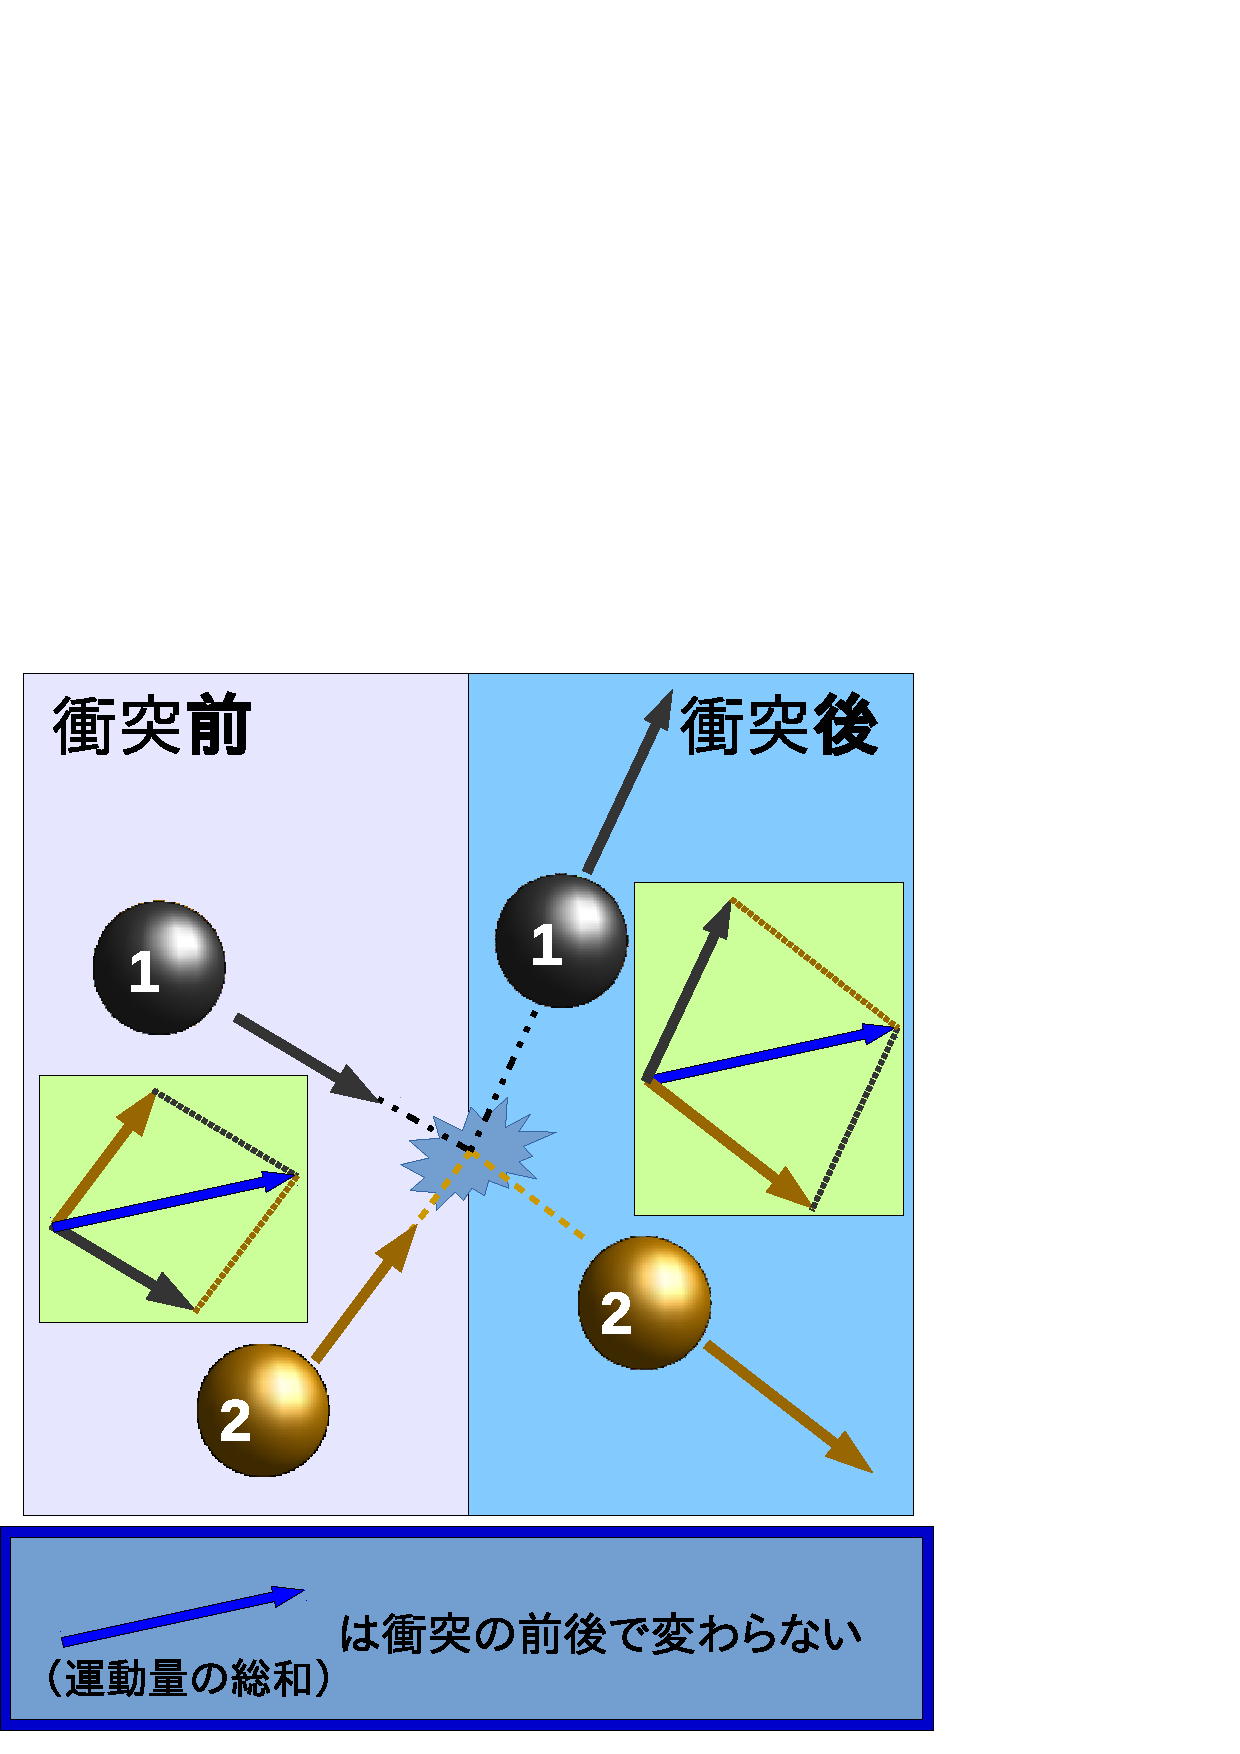
\includegraphics[keepaspectratio, width=6cm,height=8cm,clip]{P_hozonnsoku2.pdf}
                        \caption{運動量保存の法則}
                        \label{fig:Hozonasu}
                    \end{center}
                \end{figure}

            \begin{memo}{現象全体を見ることで,保存則が成立する}
                運動量保存の法則は,系の全ての物体について見渡すことで,成立している法則である.
                例えば,衝突に関係する物体全体の中の,一部の物体だけを見ているならば,
                この法則は成り立たない.1つの物体が運動量を増加させれば,
                別の物体は運動量を減少させるのである.
                この法則が意味していることは,この増加量と減少量の和が0になる ということである.
            \end{memo}

            \begin{memo}{運動方程式と運動量保存則}
                運動量保存の法則を次のように考えることもできる.すなわち,
                運動方程式$\df\textit{\textbf{P}}/\df t = \bF$ で,
                $\bF=0$ のとき,$\df\textit{\textbf{P}}/\df t =0$ である.
                従って,運動量保存の法則は運動方程式から導かれる.
            \end{memo}

            \begin{memo}{高校物理における運動量保存則}
                高校の物理学では,2つの物体の衝突を考えて,運動量保存の法則を説明した.
                より具体的な式で表現すれば,
                \begin{align}
                m_{a}\bv_{a\mbox{前}}+m_{b}\bv_{b\mbox{前}}=m_{a}\bv_{a\mbox{後}}+m_{b}\bv_{b\mbox{後}}
                \end{align}
                である.
            \end{memo}


%       %======================================================================
%       %  SubSection
%       %======================================================================
        \subsection{運動量の変化と力積}
            ある1つの物体の運動量が時間変化した場合について考える.物体が壁に当たって,
            運動方向を変化させる現象を想像するとよい.
            変化前と変化後の運動量をれぞれ,$\textit{\textbf{p}}_{\mbox{前}}$,
            $\textit{\textbf{p}}_{\mbox{後}}$ と書く.
            そして,このときの運動量の変化を $\textit{\textbf{I}}$ と書くことにすると,
                \begin{align}\label{7}
                    \textit{\textbf{I}} = \textit{\textbf{p}}_{\mbox{後}}-\textit{\textbf{p}}_{\mbox{前}}
                \end{align}
            である.

            ところで,物体が運動の方向を変化させたのだから,物体は力を受けたはずである.
            なぜなら,慣性の法則によると,
            物体に力が働かない限り,物体は等速直線運動をするからである.
            しかし,物体の運動量が変化したということは
            運動量の定義 $\textit{\textbf{p}} := m_{\mathrm{i}} \bv$ から,
            速度が変化したことになる.
            すなわち,加速度を生じたわけであり,力が加わったと解釈できる
                \footnote{
                    「加速度が生じること」と「力が加わること」は,運動方程式から,
                    同じことを意味すると言える.
                }.
            その力を $\bF$ とすると,運動方程式(\ref{6})から,
                \begin{align}
                    \frac{\df\textit{\textbf{p}}}{\df t} = \bF
                \end{align}
            をたてられる.この式の両辺を,衝突前の時間 $t_{\mbox{前}}$ から
            衝突後の時間 $t_{\mbox{後}}$ で定積分すると,
                \begin{align}\label{8}
                    \int_{t_{\mbox{前}}}^{t_{\mbox{後}}}\frac{\df\textit{\textbf{p}}}{\df t} \df t
                    &= \int_{t_{\mbox{前}}}^{t_{\mbox{後}}}\bF \df t \notag \\
                    \Leftrightarrow \int_{t_{\mbox{前}}}^{t_{\mbox{後}}}\df\textit{\textbf{p}}
                    &= \int_{t_{\mbox{前}}}^{t_{\mbox{後}}}\bF \df t \notag \\
                    \Leftrightarrow \textit{\textbf{p}}(t_{\mbox{前}})-\textit{\textbf{p}}(t_{\mbox{後}})
                    &= \int_{t_{\mbox{後}}}^{t_{\mbox{前}}}\bF \df t
                \end{align}
            となる.この式の左辺は,$\textit{\textbf{p}}_{\mbox{後}}-\textit{\textbf{p}}_{\mbox{前}}$ と
            全く同じことであるので,
            式(\ref{7})と式(\ref{8})を見比べると,
                \begin{align}
                    \textit{\textbf{I}} = \int_{t_{\mbox{前}}}^{t_{\mbox{後}}}\bF \df t
                \end{align}
            の関係を得る.この $\textit{\textbf{I}}$ のことを,\textbf{力積} という.
            つまり,運動量変化は力積 $\textit{\textbf{I}} =\int_{t_{\mbox{前}}}^{t_{\mbox{後}}}\bF \df t$
            によって生じたと考えられる.


%   %==========================================================================
%   %  Section
%   %==========================================================================
    \section{角運動量保存の法則}
        \begin{mycomment}
            回転している物体に共通する性質はあるだろうか.回転する物体として
            よく例に上がるのがコマである.また,車輪の例もよく見かける.
            回転するコマが倒れずに回転を続けられる理由や,走行中の自転車が
            安定している理由に,これから説明する角運動量保存の法則が絡んでいる.
        \end{mycomment}

%       %======================================================================
%       %  SubSection
%       %======================================================================
        \subsection{角運動}
            物体が一直線上を運動していても,ある固定された点からその物体の運動を眺めると,
            その点を中心として回転しているように見える.
            例えば,車が走っているのを見るとき,その車を1つの決まった場所から目で追うためには,
            首(あるいは目)を回転させる必要がある.
            このような回転運動のことを \textbf{角運動} という.
            (回転を表すのに角度を用いるからだろうか?)このような状況を思い浮かべつつ,
            角運動について考える.
            角運運動量を記述するには,ベクトルの \textbf{外積} の知識が必要である.

        \subsection{てこの原理}
            物体の回転の最も基本的な原理は,\textbf{てこの原理} である.
            そのままでは簡単には持ち上げられない程,重い物体があるとしよう.
            この物体を持ち上げたいとき,てこの原理が役に立つ.
            もはや,説明するまでもないだろう.図\ref{fig:teko_no_genri1}を見れば,
            分かるはずである.直接的に力を加えている部分を \textbf{力点},
            棒の回転の支えになっている点を \textbf{支点},重い物体に力がかかっている
            点を \textbf{作用点} という.
                    \begin{figure}[hbt]
                        \begin{center}
                            \includegraphicssqmid{teko_no_genri1.pdf}
                            \caption{てこの原理}
                            \label{fig:teko_no_genri1}
                        \end{center}
                    \end{figure}

            てこの原理は,重い物体を小さな力で持ち上げることを,可能にする.
            てこの原理を数式で表現してみよう.力点にかかる力を $F$ とし,
            持ち上げたい物体にかかる力(重力)を $W$ とする.
            てこの原理を使わずに,物体を持ち上げようとしても,
            加える力よりも物体の方が重く,すなわち
                \begin{equation*}
                    F < W
                \end{equation*}
            となるので,物体を持ち上げられない.

            てこの原理を使うと,上式が成り立っていても,物体を持ち上げることができる.
            支点と力点との距離を $l_{1}$,支点と作用点との距離を $l_{2}$ としよう.
            このとき,物体が持ち上がったとすると,てこの原理は
                \begin{align}
                    Fl_{1} > Wl_{2}
                \end{align}
            のように表現される.この式が成立するときに,物体を持ち上げられるの
            物体の重さ $W$ は一定であり,力 $F$ には限界値があることから,
            自由に動かせるのは ${l}_{1}$, ${l}_{2}$ しかない.
            支点から力点までの距離(${l}_{1}$)を長くし,
            支点から作用点までの距離(${l}_{2}$)を短くすることで,
            より小さい力で物体を持ち上げることが可能になる.

        \subsection{釣り合いの式}
            てこの原理の式の不等号を等号に置き換えた式を,釣り合いの式という.
                \begin{align}
                    {F}_{1}{l}_{1} = {F}_{2}{l}_{2}.
                \end{align}
            ${F}_{1}$ を物体の重さによってかかる力とし(力点),${F}_{2}$ を棒が傾かないように支える力とする(作用点).
            ${l}_{1}$ は支点と力点との距離で,${l}_{2}$ は支点と作用点との距離である.
                    \begin{figure}[hbt]
                        \begin{center}
                            \includegraphicslarge{TekonoGenri111.pdf}
                            \caption{釣り合い}
                            \label{fig:TekonoGenri111}
                        \end{center}
                    \end{figure}

%       %======================================================================
%       %  SubSection
%       %======================================================================
        \subsection{物体の回転の表現 と ベクトルの外積}
            物体が回転しているということを表現するのに,
            ベクトルの \textbf{外積} という概念を導入する.
            ここでは,このベクトルの外積について考える.

            物体が回転するということは,その軌道は円であるから,
            回転には必ずこの軌道円の中心を通る“回転の軸”が存在する.この回転の軸は直線であることは
            当たり前であって,確認するまでもない.この軸を用いて,回転の方向を表現するのである.
            回転の方向をこの軸方向にとって,回転の強さを適当に定義すれば,
            その回転の特徴を表現できる.さて,以下では回転の具体的な表現の仕方について
            考えていくことにしたいと思う.

            まず,回転の方向の決定方法である.これには回転の軸を用いることは先ほど書いたところである.
            その
            方向には正方向と負方向の2つがあるが,
            その取り決めは次の約束に従うものとされる.すなわち,回転の向きを
            \textbf{「
            速度の方向 $\bv$ の方向から,
            物体から軸へ垂線を下ろした向き($\textbf{\textit{k}}$ の方向)に
            右ねじを回して進向き」} と決めるのである.
            これを \textbf{右ねじの法則} という.
            回転の強さについてはもう少し後で考えるこにする.
                        \begin{figure}[hbt]
                            \begin{center}
                                \includegraphicssqmid{gaiseki1new.pdf}
                                \caption{物体の回転}
                                \label{fig:gaiseki1new}
                            \end{center}
                        \end{figure}

            右ねじの法則によって方向を定義されたベクトルを $\bL$ と書くことにする.
            これを,
            \begin{align}
            \bL=\textbf{\textit{k}} \times \bv
            \end{align}
            のように表現する.この式の解釈の仕方は,
            「ベクトル $\textbf{\textit{k}}$ をベクトル $\bv$ 方向へ右ねじ回して進む
            向き」のベクトルと読む.

            しかし,向きを設定したのではまだ不十分である.この $\bL$ の大きさを考える必要がある.
            そこで,大きさの定義として,「物体の速度ベクトル $\bv$ と
            垂線ベクトル $\textbf{\textit{k}}$ のなす平行四辺形の面積」を
            用いる.このような,ベクトルの大きさの定義の理由については後回しにして,
            ここではそのようなものであると考えておいてもらいたい.式でこの定義を表現すれば,
            \begin{align}
                L:=\|\bL\|=\|\textbf{\textit{k}} \times \bv\|
                =\| \textbf{\textit{k}} \| \| \bv \| \sin\theta
            \end{align}
            である.

            さて,ベクトルの大きさの具体的な
            定義を見てもらったところで,
            次にこの定義の意味の説明である.

            覚え方は,内積を定義したときには $\cos$ 関数を
            用いて定義したことと比べると,今回は
            この部分は $\sin$ 関数となっていることに注意すればよい
            ということだろうか.

            大体,物体の回転をベクトルを用いて表現すると
            以上のような感じだが,しかしこれでは感覚的過ぎる.
            そこで,この物体の回転を,ベクトルの成分を通して
            もう少し詳しく考えていくことにしたい.

%       %======================================================================
%       %  SubSection
%       %======================================================================
        \subsection{角運動量}
                \begin{figure}[hbt]
                    \begin{center}
                        \includegraphicssqmid{kaku_unndouryou2.pdf}
                        \label{fig:kaku_unndouryou2}
                        \caption{(a) 直線運動}
                    \end{center}
                \end{figure}
                \begin{figure}[hbt]
                    \begin{center}
                        \includegraphicssqmid{kaku_unndouryou1.pdf}
                        \label{fig:kaku_unndouryou1}
                        \caption{(b) 回転運動}
                    \end{center}
                \end{figure}

                物体が位置 $\br$ において,運動量 $\textit{\textbf{p}}$ をもっているとき,
                            \begin{align}
                            \bL
                            := \br \times \textit{\textbf{p}}
                            \end{align}
                で定義される $\bL$ を原点の周りの \textbf{角運動量} という.
                物体の角運動量 $\bL$ が0でない値をとるとき,その物体は回転運動
                をしていると言える.

%       %======================================================================
%       %  SubSection
%       %======================================================================
        \subsection{角運動の方程式}
                回転運動している物体の運動方程式を考えてみよう.

                角運動量 $\bL$ を時間微分すると,
                    \begin{align}\label{9}
                        \frac{\df\bL}{\df t}
                        = \frac{\df\br}{\df t} \times \textit{\textbf{p}}
                        +\br \times \frac{\df\textit{\textbf{p}}}{\df t}
                    \end{align}
                となる.ここで,式(\ref{9})の第1項の運動量 $\textit{\textbf{p}}$ は
                    \begin{align}
                        \textit{\textbf{p}} = m\bv=m\frac{\df\br}{\df t}
                    \end{align}
                である.これを用いて,
                    \begin{align}\label{9_1}
                        \frac{\df\bL}{\df t}
                        = \frac{\df\br}{\df t} \times m\frac{\df\br}{\df t}
                        +\br \times \frac{\df\textit{\textbf{p}}}{\df t}
                    \end{align}
                となるが,ベクトルの外積の性質
                (任意のベクトル $\bA$ に対して $\bA \times \bA=0$ が成り立つ)
                を考慮すると,
                    \begin{align}
                        \frac{\df\br}{\df t} \times m\frac{\df\br}{\df t}
                        =m\left( \frac{\df\br}{\df t} \times \frac{\df\br}{\df t} \right)=0
                    \end{align}
                となってしまうので,式(\ref{9_1})の第1項は 0 にってしまい,結局,
                    \begin{align}
                        \frac{\df\bL}{\df t} = \br \times \frac{\df\textit{\textbf{p}}}{\df t}
                    \end{align}
                と計算される.さらに,運動量を用いた運動方程式(\ref{6})の関係から,
                    \begin{align}\label{10}
                        \frac{\df\bL}{\df t} = \br \times \bF
                    \end{align}
                を得る.ここで,原点の周りの \textbf{力のモーメント} $\bN$を
                    \begin{align}\label{12}
                        \bN := \br \times \bF
                    \end{align}
                と定義すると,式(\ref{10})は
                    \begin{align}\label{11}
                        \bN = \frac{\df\bL}{\df t}
                    \end{align}
                と書ける.式(\ref{11})は,運動量を用いた運動方程式(\ref{6})と同じ形の式になっている.
                ($\bN$ → $\bF$,
                $\bL$ → $\textit{\textbf{p}}$ とするとわかる.)
                従って,式(\ref{11})は角運動についての運動方程式であると言える.
                力のモーメント $\bN$ は,角運動を引き起こす力である.
                すなわち,$\bN$ は回転運動を引き起こす力であると言える.
                このように回転力を起こす $\bN$ は \textbf{トルク} ともよばれる.

%       %======================================================================
%       %  SubSection
%       %=====================================================================
        \subsection{角運動量保存則}
                運動量保存則を考えたときに,
                「外部から力 $\bF$ が加わらない限り,全物体の運動量の総和は一定である」
                ということを確認した.
                角運動量についても同様な法則が成り立っていて,これを \textbf{角運動量保存の法則} という.
                または略して,\textbf{角運動量保存則} という.
                では,角運動量保存則 を式で表すことを考える.外力が働かないことから,$\bF=0$ であって,
                これを力のモーメントの定義式(\ref{12})に代入することで,
                $\bN := \br \times 0 =0$ を得る.よって,
                この $\bN=0$ を角運動についての運動方程式(\ref{11})に代入して,
                \begin{equation*}
                    \frac{\df\bL}{\df t} = 0
                \end{equation*}
                となる.この式は,外力が働かなければ,角運動量の時間変化がないことを示している.
                つまり,時間によらずに一定値をとることを意味する.従って,式(\ref{13})
                は角運動量保存則を表現した式であると言える.
                    \begin{myshadebox}{角運動量保存則}
                            位置ベクトル $\br$ にある物体に外力が働いていない場合($\bF=0$),
                            角運動量 $\bL$ は時間経過にかかわらず,一定に保たれる.
                            \begin{align}\label{13}
                                \frac{\df\bL}{\df t} = 0
                            \end{align}
                    \end{myshadebox}

                角運動量保存則を積分すれば,定ベクトルを得る.実際に確かめてみよう.
                角運動量保存則は 式(\ref{13})により $\df\bL/\df t = 0$ である.
                この角運動量 $\bL$ は $\bL
                := \br \times \textit{\textbf{p}}$ で定義される量であった.従って,
                角運動量保存則は
                    \begin{align}
                        \frac{\df \left(\br \times \textit{\textbf{p}}\right)}{\df t} = 0
                    \end{align}
                と表現しても同じことである.そして,両辺を時間で積分して,
                    \begin{align}
                        \int\left(\frac{\df \left(\br \times \textit{\textbf{p}}\right)}{\df t}\right) \df t = \bC
                    \end{align}
                ここに, $\bC$ は定ベクトルである.よって,
                    \begin{align}
                        \br \times \textit{\textbf{p}}=\bC
                    \end{align}
                を得る.この式は,位置 $\br$ が原点から遠くなるほど,運動量は小さくなることを意味している
                逆にいえば,原点に近いほど,運動量は大きくなるのである.

                例えば,スケーターの回転を考えてみる.この場合の座標原点は体の重心にとる.
                スケーターが自身の腕を大きく広げたときほど ゆっくりと回転している のは,手の位置 $\br$ が
                体の重心からより遠くなるためである.すなわち,これは $\br$ が
                大きくなることを意味する.しかし,特に外力が働かないので,(氷との摩擦は無視する)
                角運動量保存の法則 $\br \times \textit{\textbf{p}}=\bC$ が成立している.
                従って,運動量 $\textit{\textbf{p}}$ が小さくなるのである.
                というか,運動量を小さくすることで,角運動量保存則を満たそうとするのである.

                腕を縮めると回転が速くなるのは,この逆で,手の位置 $\br$ が
                体の重心に近づくからである.従って,角運動量保存則を満たすために
                運動量 $\textit{\textbf{p}}$ を大きくするのである.


%   %==========================================================================
%   %  Section
%   %==========================================================================
    \section{力学的エネルギー保存の法則}
%       %======================================================================
%       %  SubSection
%       %======================================================================
        \subsection{仕事}\label{shou_sigoto}
%       %======================================================================
%       %  SubsubSection
%       %======================================================================
        \subsubsection{1次元上の仕事}
                まず簡単に,一方向のみに限定して考える.その一方向を,$x$ 方向とする.
                さて,物体に外力 $F_{x}$ を加えて, $x$ 方向に $\Delta x$ だけ変位させたとしよう.
                物体の移動は,物体に与えた外力 $F_{x}$ とその変位の大きさ $\Delta x$ できまる.
                この移動は,物体が「仕事」をされたから,生じたものであると考える.仕事は,記号 $W$ で
                表され,次式よって定義される.
                    \begin{equation*}
                        W  :=  F_{x} \Delta x.
                    \end{equation*}
                単位は上の定義式から,[Nm] である.仕事の単位を表す記号は [J] が使われる.
                つまり,[J] = [Nm] である.単位については後で改めて,記述しよう.

                「仕事」という概念を導入することで,物体の移動を考えやすくなる.物体が
                移動したということは,物体に外力が働いて,変位したということであるが.
                その力の方向と変位の方向を考慮する必要がない場合,
                    \begin{equation*}
                        \mbox{物体は「仕事」} W \mbox{をされた.}
                    \end{equation*}
                あるいは,視点を変えて,
                    \begin{equation*}
                        \mbox{「仕事」} W \mbox{をした.}
                    \end{equation*}
                と表現できる
                    \footnote{
                        もう少し学習を進めると,「エネルギー」という概念が導入される.この「エネルギー」を
                        説明するために,「仕事」が使われるのであるが,実は後で記述するように,仕事と
                        エネルギーには,表と裏のような関係がある.「エネルギー」は,物理学で最も重要な
                        概念の1つである.
                    }.
                一方向だけで考えられるならば仕事の定義は上の式で十分である.

%       %======================================================================
%       %  SubsubSection
%       %======================================================================
        \subsubsection{3次元内の仕事}
                物体に力を加えたときの物体の変位の方向は,必ずしも,その力の方向であるとは限らない.
                変位も3次元を考えることができて,一方向だけではない.
                例えば,重い荷物を引っ張るとき,真横に力を加えるのではなく,少し上向きに引っ張ることが
                多い.このとき物体は地面から離れず,ただ地面に引きずられるという場合が起こり得る.
                そのとき,力が物体にした仕事は,その力の全てではなく,地面に対して平行な力の成分
                しか仕事をしていない.上向きの成分は,物体が上に上がっていないので,仕事はしていないのである.
                このような場合でも仕事を定義できるように導入されるのが,「なす角」である.
                ここでは,なす角を導入し,$\theta$ で表すことにしよう.
                「なす角」と聞いて,すぐにベクトルの内積が頭に浮かぶと思う.そうベクトルの内積を用いて,
                仕事を定義するのである.

                なす角 $\theta$ を導入すると,力を加えた方向と異なる向きに物体が移動したときにも,
                仕事を定義できるのである.
                    \begin{figure}[hbt]
                        \begin{center}
                            \includegraphicssqmid{sigoto_nasukaku.pdf}
                            \caption{力と仕事(3次元)}
                        \end{center}
                    \end{figure}

                少しかしこまった形で,なす角を導入しよう.
                物体が一定の力 $\bF$ で,\underline{直線距離} $\Delta \textit{\textbf{s}}$ だけ変位したとき,
                \textbf{仕事} $W$を次式で定義する.
                    \begin{align}
                        W:=\bF\cdot\Delta \textit{\textbf{s}}=F\Delta s \cos \theta
                    \end{align}
                ここに,$\theta$ は $F$ と $\Delta s$ の \textbf{なす角} (図\ref{fig:nasu}参照)である.
                    \begin{figure}[hbt]
                        \begin{center}
                            \includegraphicssqmid{nasu.pdf}
                            \caption{力 $\bF$ と変位 $\Delta\textit{\textbf{s}}$ のなす角 $\theta$ }
                            \label{fig:nasu}
                        \end{center}
                    \end{figure}


%       %======================================================================
%       %  SubsubSection
%       %======================================================================
        \subsubsection{仕事の単位}
                仕事の単位は[J]
                    \footnote{
                        ジュールと読む.仕事と熱量の関係を研究した物理学者Jouleの頭文字である.
                    }
                が用いられる.上の仕事の定義からわかるように,仕事の単位はSI単位系
                    \footnote{
                        SI単位系:基本単位として[m](メートル),[Kg](キログラム),[s](セコンド),[A](アンペア)
                        を用いる単位系のこと.\date 現在,SI単位系は国際標準となっている.
                        $\longrightarrow $昔はcgs単位系([cm](センチメートル),[g](グラム),[s])もよく使われていたみたいである.
                        古い教科書を見てみると,cgs単位系で書かれているもの多い.
                    }
                で,
                    \begin{align}\label{eq:Jule}
                        \mathrm{
                            [J]=[Nm]=[kgm^{2}/s^{2}]
                        }
                    \end{align}
                である.

%       %======================================================================
%       %  SubsubSection
%       %======================================================================
        \subsubsection{一般的な仕事の定義}
                次に,物体が 位置によって異なる力 $\bF(\br)$ で,
                \underline{曲線} $\br$ に沿って変位したときの仕事を考える.
                曲線の微小部分 $\df\br$ では力は一定と考えられる.
                よって,この微小部分 $\df\br$ における仕事は
                $\bF(\br) \cdot \df\br$ と書ける.
                すなわち,微小部分での仕事を積分すると,求める仕事 $W$ を得る.従って,位置 $\br_{A}$ か
                ら 位置 $\br_{B}$
                変位が曲線をとるときの仕事は
                    \begin{align}
                        W:=\int_{\br_{A}}^{\br_{B}}
                        \bF(\br) \cdot \df\br
                    \end{align}
                と定義できそうである.しかし,\textbf{これでは不十分である}.なぜなら,位置 $\br_{A}$ から
                位置 $\br_{B}$ までの曲線は無限に作れるからである.というのも
                そのような曲線によって,仕事が異なるからである.これは当たり前のだろう.
                曲線が変わってしまえば,物体の変位する“道のり”が長くなったり,短くなったりするのだから,
                当然,仕事もこの曲線によって異なると考えられる.
                そこで,位置 $\br_{A}$ から
                位置 $\br_{B}$ までの
                この曲線を指定する.それを \textbf{経路} という.位置 $\br_{A}$ から
                位置 $\br_{B}$ までの経路 $C$ に沿って,変位したときの仕事は,次のように書く.
                        \begin{myshadebox}{仕事の定義}
                            経路 $C$ に沿って物体を動かす際の仕事 $W$ を,次式で定義する.
                            \begin{align}
                                W=\int_{C}\bF(\br) \cdot \df\br.
                            \end{align}
                        \end{myshadebox}
                    \begin{figure}[hbt]
                            \begin{center}
                                \includegraphicssqmid{sensekibun_shukaisekibun_000.pdf}
                                \caption{点Aから点Bまで}
                                \label{fig:sigoto_keiro1}
                            \end{center}
                    \end{figure}


                特に,この\underline{経路が閉曲線である場合},
                    \begin{align}
                        W=\oint_{C}\bF(\br) \cdot \df\br
                    \end{align}
                と書かれることがある.\ref{subsec:hozonryoku_to_shukaisekibun} 節も参照.
                    \begin{figure}[hbt]
                            \begin{center}
                                \includegraphicssqmid{sensekibun_shukaisekibun_003.pdf}
                                \caption{始点と終点が同じ}
                                \label{fig:keiro_loop}
                            \end{center}
                    \end{figure}

                \begin{memo}{注意}
                    もう一度書いておくが,仕事を計算するときは,最初に経路を指定することが必要である.
                    今までの話だと,仕事が経路によって異なってしまうのだから,
                    このような定義では十分でないと思われるかもしれないが,
                    ここで仕事という概念を定義したのは,
                    この仕事が経路によらないような力を導入したいためである.
                    そのような力の例として,最も簡単な例に,地表付近の
                    物体が受ける力 $m\textit{\textbf{g}}$ がある.
                    どのように示されるかは以下で考えることである.
                \end{memo}

%       %======================================================================
%       %  SubSection
%       %======================================================================
        \subsection{エネルギーについて}
%           %==================================================================
%           %  SubsubSection
%           %==================================================================
            \subsubsection{エネルギー}
                物体が外部から仕事を受けたとき,その物体は \textbf{エネルギー} を
                与えられたという.例えば,人間が物体を高さ $h$ だけ上にあげれば,
                物体は人間による外力から仕事されたことになり,
                従ってエネルギーを外力から与えられたということになる.

                数式っぽく表現すれば以下のようなるだろう.すなわち,
                    \begin{center}
                        『外力が物体に仕事をする=物体は外力を受けることにより,エネルギーを与えられる.』
                    \end{center}
                つまり,「エネルギーをもつ」ということは「仕事ができる状態にある」
                ということと同じである.
                従って,\textbf{仕事とエネルギーは同じ単位をもつ}.
                エネルギーと仕事の関係は視点の違いこそあるけれど,
                同等なものであると言える.「仕事」という時は外力を主眼と考えるときであり,
                「エネルギー」という時には物体を主眼として考えていると言える.
                    \begin{figure}[hbt]
                        \begin{center}
                            \includegraphicssqmid{ENERGY_1.pdf}
                            \caption{仕事とエネルギー}
                            \label{fig:ENERGY_1}
                        \end{center}
                    \end{figure}

                                仕事をする側はエネルギーが減り,仕事をされる側はエネルギーが増えるのである.
                                これを式で表現してみよう.摩擦などの外的要因はない理想状態で考える.

                                まず,仕事をする側に着目する.$W$ だけ仕事をした場合,
                                もともと持っていたエネルギーを $E_{a0}$ とすると
                                        \footnote{
                                                $E_{a0}$ の $a$ は仕事"する"側で,能動を意味する英単語 active の頭文字を使った.
                                                0は仕事する前を示すものとし,1を仕事した後を示すものとして使う.
                                                仕事"される"側は,受動を意味する英単語 passive の $p$ を使う($E_{p0}$,$E_{p1}$).
                                        },
                                仕事した後のエネルギー $E_{a1}$ は,
                                        \begin{equation*}
                                                E_{a1} = E_{a0}-W.
                                        \end{equation*}

                                一方で,仕事をされた方は $W$ だけのエネルギーが入ってくる.
                                仕事される側のもともと持っていたエネルギーを $E_{p}$ とすると,
                                仕事をされた後のエネルギー $E_{p1}$ は,
                                        \begin{equation*}
                                                E_{p1} = E_{p0}+W.
                                        \end{equation*}
                                つまり,
                                        \begin{align}
                                                E_{a1} + E_{p1} &= (E_{a0}-W) + (E_{p0}+W)  \notag \\
                                                                &= E_{a0} + E_{p0}
                                        \end{align}
                                と計算され,仕事する前後では,"する側" と "される側" の全系で考えた場合,
                                全体的なエネルギーの変化はないことがわかる.実験的にも,摩擦などを極力小さくした場合,
                                上式に反した結果はない.こうなると,これを逆手に取り,
                                「物体の運動状態が変化しても,総エネルギーは変化しない」という仮説を立てたくなる.
                                実際,\textbf{エネルギー保存の法則} として,この仮説は物理法則の重要な1つに格上げされる.

                                ただ,エネルギーと言っても,運動やポテンシャルに関するもの,熱に関するもの,電磁気に関するものなどと,
                                様々な形態がある.すごいことに,どんな形態でも,エネルギー保存の法則が成立することが確かめられている
                                (実験事実).この法則が各エネルギー形態でどう表現されるかは非常に興味のあることである.
                                以下では,特に力学に関するエネルギー(運動エネルギーと位置エネルギー)を中心に,エネルギーという
                                概念について少し詳しく勉強していくことにしよう.

%           %==================================================================
%           %  SubsubSection
%           %==================================================================
            \subsubsection{エネルギーの種類}
                先にも書いたが,物体のもつエネルギーには,様々な形態がある.例えば,運動エネルギー,
                ポテンシャル$\cdot$エネルギー,熱エネルギー,電磁気的エネルギー 等がある.これらは全てエネルギーである.

                なぜこういうことが言えるかというと,一言で言うと,そう考えると意味のある理論が作れるからということになる.
                最初は,物体の運動に関すること,熱に関すること,電気に関すること,磁気に関すること,と言ったように,
                物理分野の別々の側面から現象が観測されていて,そもそもエネルギーという抽象的な概念はなかった.
                各分野の発展に伴い,それらに共通部分が見出されてくることも多い.その1つに,エネルギーがある.
                各分野がエネルギーという概念により有機的につながることがわかったのである.
                しかし,エネルギーとは人が様々な物理現象の研究から炙りだした抽象概念であり,"エネルギーそのもの" というものは
                ない.エネルギーを見るには,電気や熱などの具体的な現象を見るしかない.

                なので,勉強する際も,様々に現れる具体的なエネルギー形態を一つずつ確かめながら,
                エネルギーという概念の把握に努めたい.
                抽象的なエネルギーとはこうだ,と定義してから各分野でエネルギーがどう現れるかを
                議論したいところだが,まず現象を知らないとエネルギーについてのイメージを持ちようがないのだ.
                面倒だが,具体例を逐一見ていくしかない.

                どの形態のエネルギーも等しく重要な概念であり,全てのエネルギー形態について調べる必要があるが,
                以下ではその最も基本であるとされる,運動エネルギーと位置エネルギーについて考える.

%           %==================================================================
%           %  SubsubSection
%           %==================================================================
            \subsubsection{「エネルギー」のイメージ}
                                とはいっても,何のイメージもなしにエネルギーについて勉強するのはつらい.ジレンマだ.
                                ここでは,その概念の重要さについて記述することで,学習意欲を少しでも高めたい.

                エネルギーの概念は簡単につかめるものではない.少しもどかしいかもしれないが,とりあえずはエ
                ネルギーとはこんなものだと思って,先に進んでしまうことである.その進んだ先で,違った形の色
                々なエネルギーを見ることになるだろう.これらの色々な形のエネルギーをみて,初めて,エネルギ
                ーという感覚がつかめていくことだろう.ここは先人の知識を信じて先に進もう.エネルギーという
                概念はもうとっくに定着しているものであり,覆ることはないのだから…

                いや,むしろエネルギーそのものを,具体的に想像することはできない.エネルギーを知っていると
                いうかもしれないが,それは熱だとか電気だとか,何か物理的な現象となって生じているので,その
                ものを見てはいない.ではなぜ,エネルギーという概念が生まれたのだろうか.
                物理学には \textbf{保存則} というキーワードがある.保存則とは,例えば,ある現象の前後で変化
                しない量が存在するとき,この量は保存するといい,この法則のことを保存則という.
                また \textbf{保存量} とは,時間的に増えたり減ったりしない,何か本質的な量のことをいう.昔の
                人々は,物理法則を考えるにあたって,保存量を見つけ出すことにも力を注いでいた.この保存量の
                一つがエネルギーである.つまり,エネルギーは保存量として導入されたものである.

                実をいうと,エネルギーが保存することを実験で確かめる必要があるのだが,実験には誤差がつきも
                のであるので,厳密にはわからない.それにもかかわらず,エネルギーは保存すると言えるのは,そ
                の他の実験との矛盾がなく,むしろエネルギーが保存することでいろいろな現象を説明することがで
                きるからである.


%       %======================================================================
%       %  SubSection
%       %======================================================================
            \subsection{ポテンシャル$\cdot$エネルギー}
%           %==================================================================
%           %  SubsubSection
%           %==================================================================
            \subsubsection{高さ(位置)によるエネルギーの違い}
                地表面を位置の基準に取る.$z$ 座標を鉛直上向きを正にとる.
                質量 $m$ の物体を地表面から,高さ $h$ のところまで,
                垂直にではなく,クネクネ と曲がった経路 $C$ でもち上げられたときの仕事を考える.
                図\ref{fig:PE_fig}を参照.
                    \begin{figure}[hbt]
                        \begin{center}
                            \includegraphicssqmid{PE_fig.pdf}
                            \caption{物体の移動のある瞬間}
                            \label{fig:PE_fig}
                        \end{center}
                    \end{figure}

                このとき,持ち上げるのに要する力 $\bF(\br)$ は必ずしも鉛直上向きではない.
                力に負の符号をつけたのは,鉛直下向きを正とした
                ことによる.鉛直下向きの重力に逆らって 物体を持ち上げるのだから,
                負の符号がつくのである.
                この力を鉛直な成分 $\bF
                (\br)_{\perp}$
                と地面に水平な成分 $\bF
                (\br)_{\parallel}$ に分解する.
                    \begin{align}
                        \bF(\br)=\bF_{\perp}(\br)
                        +\bF_{\parallel}(\br)
                    \end{align}
                この力を経路に沿って線積分する.
                    \begin{align}
                        W &= \int_{C}\left(\bF_{\perp}(\br)   + \bF_{\parallel}(\br) \right) \cdot \df\br \notag \\
                          &= \int\bF_{\perp}(\br)\cdot \df\br + \int\bF_{\parallel}(\br) \cdot \df\br
                    \end{align}
                地表付近における,物体の地球から受ける力は,$m\textit{\textbf{g}}$ である.
                これを上式に代入するのだが,
                重力加速度の向きは鉛直方向を向いているので,水平方向との内積は0になる.(
                力の 鉛直成分 と 変位の水平移動方向 のなす角は
                $\frac{\pi}{2}$である.)従って,第1項のみが残って,
                    \begin{align}
                        W=-\int m\textit{\textbf{g}}\cdot \df\br
                    \end{align}
                となる.さらに,外力の鉛直方向と重力加速度とのなす角は $\pi$ であることを考慮し,
                $\textit{\textbf{g}} \cdot \df\br=g\df r \cos \pi=-g\df r$ の関係から,
                    \begin{align}
                        W=-mg\int \df r.
                    \end{align}
                内積計算を行ったので,ベクトル演算が消え,スカラー積となったことに注意.
                ここで,垂直方向は0になっていたために,上の $dr$ は鉛直成分を考えばよく, $h=\int \df r$ であるので,
                    \begin{align}
                        W=-mgh
                    \end{align}
                を得る
                    \footnote{
                        意味を強調するのであれば,$W=m(-g)h$ と書いたほうがよい.
                        質量 $m$ は常に正であるし,高さ $h$ は地表から空へと向かう
                        向きを正としているから,この場合は正の値をとるはずである.重力加速度 $\bg$ の向きは逆向きの
                        外力 $\bF_{\mbox{外力}} = -m\bg$ を加えることにより,
                        距離(ここでは高さ)$h$ だけ移動させ($W=m(-g)h$ の仕事をしたことになる),
                        物体にポテンシャル$\cdot$エネルギー $U=m(-g)h$ を与えたのだ.与えたエネルギーは仕事と
                        等しく,$W=U$ である(ポテンシャル$\cdot$エネルギーの定義).
                        物体に仕事 $W$ を与えたことにより,物体にエネルギー $U$ が溜められたと
                        いうイメージだ.見方を変えれば $W-U=0$ で,物体に与えた仕事 $W$ と
                        溜まったエネルギー $U$ の正味の和は0であり,物体のエネルギーは勝手に
                        湧きだしたものではなく,外力のみによって与えられたと捉えることもできる.
                    }.
                この計算結果から,いかなる経路でも,物体を高さ $h$ まで持ち上げるのに
                必要な仕事は,$W=-mgh$ であることがわかる.
                なぜなら,力がどんな方向に向いていようが,
                地面に垂直な成分 と 地面に平行な成分 に分割することができ,地面に平行な成分は
                全く仕事には関与せずにいるからである.
                力の 鉛直成分 と 変位の水平移動方向 の内積がいつも 0 であることからこのことがいえる.
                力が位置に依存するにしても,高さが決まってしまえば,上の計算からどんな場合でも
                 $-mgh$ の結果を得てしまうことは明らかである.

%           %==================================================================
%           %  SubsubSection
%           %==================================================================
            \subsubsection{エネルギーの値が負であるのはなぜか}
                ポテンシャル$\cdot$エネルギーには負の符号が付いている.
                これは,負の値をもつエネルギーを意味するのだろうか.
                答えは否.エネルギーが負の値を取るなんて考えられないのだから
                    \footnote{
                        ただし,量子力学を学習していくと,量子力学と特殊相対性理論
                        とを統一すると(最初にディラックが成功した),負の値をとる
                        エネルギーが生じることを発見した.実際に,負のエネルギーを
                        認めると,陽電子の存在が予言され,これは実際に実験的に確か
                        められている(ディラックはノーベル賞を得ている).

                        ここで言う負の符号と,ディラックの負値のエネルギーとは全く
                        概念が異なる.負値のエネルギーについては,相対論的量子力学
                        を学ぶ際に,出会うことになる.

                        まあ,細かいことは後回しにして,話を先に進めよう.
                    }.
                では,この負の符号はどういうことかというと,単に重力加速度 $g$ の
                向きの定義によるものである.
                物体を持ち上げるには,重力加速度に逆らって仕事を加えないと
                ならないが,重力加速度の向きを鉛直下向きを正方向としたので,
                仕事する方向が負になってしまうのである.

                高さ $h$ に位置する物体は,仕事 $W=-mgh$ を受けて,地上から上がったのである.
                重力に逆らって,高さ $h$ までもち上げたのだから,
                重力は物体を元も位置(地表)に戻そうとする.
                従って,この物体は,$-mgh$ の仕事をし得る状態にある.
                $-mgh$を,地表付近の重力の \textbf{ポテンシャル$\cdot$エネルギー} という.
                または \textbf{位置エネルギー} ともよばれる.
                地表から高さ $h$ にある物体は「潜在的に」$-mgh$ の仕事をし得ると考えるのである
                    \footnote{
                        「負の仕事をし得る」という表現は何か不可解であるならば,「正の仕事を\textbf{される}」
                        と表現しても同じことである.これは単に言葉による表現の仕方の違いであって,
                        その内容は全く同等なものである.
                    }.

%           %==================================================================
%           %  SubsubSection
%           %==================================================================
            \subsubsection{ポテンシャル$\cdot$エネルギーの定義}
                改めて,地表付近における重力のポテンシャル$\cdot$エネルギー $U$ を定義する.
                    \begin{align}
                        U := -mgh
                    \end{align}
                ここに,$m$ は質量であり,$g$ は重力加速度であり,$h$ は高さである.
                    \begin{figure}[hbt]
                        \begin{center}
                            \includegraphicssqmlrg{itienerugi.pdf}
                            \caption{高さ $h$ でのポテンシャル$\cdot$エネルギー}
                            \label{fig:itienerugi}
                        \end{center}
                    \end{figure}

%           %==================================================================
%           %  SubsubSection
%           %==================================================================
            \subsubsection{一般的なポテンシャルエネルギー}
                実は今まではポテンシャル$\cdot$エネルギーとして
                地表付近の重力によるものを想定してきたが,
                ポテンシャル$\cdot$エネルギーとはこれだけではなく,
                電気的なポテンシャル$\cdot$エネルギーというものも考えられる.
                これを \textbf{電位} というが,詳細は電磁気学の部分で
                確認することとする.とりあえず,ここでは,そのような概念もあるのだ
                と思ってくれればよい.ここで言いたかったことは,
                ポテンシャルが位置エネルギーだろうが電位だろうが,
                エネルギー保存の法則を満たすということである.エネルギー保存の法則を
                もっと一般的に捉えられるということを理解してほしい.

%       %======================================================================
%       %  SubSection
%       %======================================================================
        \subsection{運動エネルギー}
            \begin{mycomment}
                運動エネルギーをいきなり定義しても
                わけがわからないと思うので,とりあえず感覚的に理解できるような形で
                説明する.
            \end{mycomment}

%           %==================================================================
%           %  SubsubSection
%           %==================================================================
            \subsubsection{物体を高いところから落とすと$\cdots$}
                前の項目において,地表付近のポテンシャル$\cdot$エネルギーは $-mgh$ であることが分かった.
                ここで,$m$ は質量を表し,$h$は高さを表す.
                今,高さ $h$ に存在する物体が静に落下し(初速度は 0),
                高さ $h-\Delta h(<h)$ に変化したとする.
                このときの位置エネルギーは $-mg\left(h-\Delta h\right)$ である.
                高さが $h$ から$h-\Delta h$に変化したことで,
                位置エネルギーがどれだけ変化したかを考えれば,$-mg\Delta h$ である.
                $-mg\Delta h$のエネルギーはどこにいってしまったのだろうか.
                実は,\textbf{運動エネルギー} に変わったのである.つまり\underline{速度をもった}のである.
                図\ref{fig:KE_fig}参照.
                    \begin{figure}[hbt]
                        \begin{center}
                            \includegraphicssqmlrg{rakka_k.pdf}
                            \caption{運動エネルギーの説明}
                            \label{fig:KE_fig}
                        \end{center}
                    \end{figure}

%           %==================================================================
%           %  SubsubSection
%           %==================================================================
            \subsubsection{位置エネルギーから運動エネルギーへ}
                以下では,この運動エネルギーについて考える.
                位置が変位して速度が生まれたのだから,位置と速度の関係式が使える.
                位置と速度の関係式は,
                    \begin{align}
                        2\textit{a}\left(\textit{r}-\textit{r}_{0}\right)
                        =\textit{v}^{2}-{\textit{v}_{0}}^{2}
                    \end{align}
                のように表現される.
                但し,ここでは鉛直方向を考えているので,大きさだけを考えている.
                この式に,今の条件
                (初速度 $\textit{v}_{0}=0$ ,初期位置$\textit{r}_{0}=h$
                ,重力加速度$\textit{a}=\textit{g}$ ,現在の位置$r=h-\Delta h$)
                を代入して,
                    \begin{align}
                        2\textit{g}\cdot\left(-\Delta h\right)
                        =\textit{v}^{2}
                    \end{align}
                となる.従って,
                    \begin{align}
                        \Delta h = -\frac{\textit{v}^{2}}{2g}
                    \end{align}
                を得る.これを位置エネルギーの変化量 $-mg\Delta h$ に代入すると,
                    \begin{align*}
                        -mg\Delta h =- mg\left(-\frac{\textit{v}^{2}}{2g}\right) = \frac{1}{2} m {\textit{v}^{2}}
                    \end{align*}
                すなわち,
                    \begin{align}
                        -mg\Delta h = \frac{1}{2} m {\textit{v}^{2}}
                    \end{align}
                を得る.
                これはつまり,
                            \textbf{
                            位置エネルギーの変化が鉛直下向きの速度をもつ 運動エネルギー に変換された
                            }ことを意味する.
                この量はポテンシャル$\cdot$エネルギーと等価な量である.

%           %==================================================================
%           %  SubsubSection
%           %==================================================================
            \subsubsection{運動エネルギーの定義}
                上の説明から,物体の持つポテンシャル$\cdot$エネルギーが,
                落下等の現象によって,速度に関するエネルギーに変換されることが
                わかった.落下によって,ポテンシャル$\cdot$エネルギーが失われ,
                速度に関するエネルギーに変わったので,この新しいエネルギーに
                名前を付けないとならない.

                そこで,運動エネルギー $T$ を定義する.
                    \begin{align}
                        T :=  \frac{1}{2} m {\textit{v}^{2}}
                    \end{align}

                ここで,このように定義した運動エネルギーは
                エネルギーの単位[J]をもつかどうかを確かめておく.
                質量の単位は[kg],速さの単位は$\mathrm{[m/s]}$であるから,
                    \begin{align}
                        \mathrm{ [kg\cdot (m/s)^{2}]} &= \mathrm{[kg\cdot m^{2}/s^{2}]      } \notag \\
                                                      &= \mathrm{[(kg\cdot m/s^{2})\cdot m] } \notag \\
                                                      &= \mathrm{[N\cdot m]=[J]             }
                    \end{align}
                となって,確かにエネルギーの単位をもつことがわかる.「エネルギーを得る」ということは
                仕事をされるということであり,エネルギーの単位は仕事の単位と等しい.
                つまり,エネルギーの単位も [J] である.確かに運動エネルギーの単位は[J]であるとが確かめられた.

%           %==================================================================
%           %  SubsubSection
%           %==================================================================
            \subsubsection{運動量と運動エネルギーの関係式}
                当たり前ではあるが,運動エネルギーについては,
                ここで定義したものしか存在しない.運動エネルギーが
                運動量を用いて $T=p^{2}/2m$ と書かれる
                こともあるだろうが,これは,$\textit{\textbf{p}}=m\bv$ の関係式を思い出せば,
                $T=mv^{2}/2$ 全く同じことを言っているとわかる(代入してみればよい).
                    \begin{align}
                        T=\frac{1}{2}mv^{2}=\frac{m}{2m}mv^{2}=\frac{(mv)^{2}}{2m}=\frac{p^{2}}{2m}.
                    \end{align}

                運動エネルギーは,運動量と速度のどちらでも表現可能だが,その違いは
                単に表記の違いだけであって,2種類の運動エネルギー存在するわけではない.


%       %======================================================================
%       %  SubSection
%       %======================================================================
        \subsection{力学的エネルギー保存の法則}
%           %==================================================================
%           %  SubsubSection
%           %==================================================================
            \subsubsection{高校生向けの説明}
                ポテンシャル$\cdot$エネルギー $U$ と運動エネルギー $T$ の和を \textbf{力学的エネルギー} という.
                力学的エネルギーを $E$ で表現する.
                    \begin{myshadebox}{力学的エネルギーの定義}
                        力学的エネルギー $E$ を,次式で定義する.
                        \begin{align}\label{eq:KE}
                        E := T + U
                        \end{align}
                    \end{myshadebox}


                このように定義された力学的エネルギーをもつ物体は,
                外力が働かない限り,
                保存する.
                「保存する」というのは「ある一定の値を保つ」ということである.
                このことを \textbf{力学的エネルギー保存の法則} という.
                力学的エネルギー保存の法則を表す式を導出する.そのために,もう一度,式(\ref{5})を使う.
                簡単のために,運動を一方向にかぎって考える.
                最初の状態(速度$v_{1}$,位置$h_{1}$)から,後の状態(速度$v_{2}$,位置$h_{2}$)に変化しとする.
                すると,
                    \begin{align}
                        2\textit{g}\left(\textit{h}_{2}-\textit{h}_{1}\right)
                        ={\textit{v}_{2}}^{2}-{\textit{v}_{1}}^{2}
                    \end{align}
                という式が立てられる.この式の両辺に,質量 $m$ を掛けて整理すると,
                    \begin{align}
                        2mg\left(\textit{h}_{2}-\textit{h}_{1}\right)
                        &= m{\textit{v}_{2}}^{2}-m{\textit{v}_{1}}^{2} \notag \\
                        \Leftrightarrow\quad 2mgh_{2}-2mgh_{1}
                        &= m{\textit{v}_{2}}^{2}-m{\textit{v}_{1}}^{2} \notag \\
                        \Leftrightarrow\quad mgh_{2}-mgh_{1}
                        &= \frac{1}{2}m{\textit{v}_{2}}^{2}-\frac{1}{2}m{\textit{v}_{1}}^{2} \notag \\
                        \Leftrightarrow\quad \frac{1}{2}m{\textit{v}_{1}}^{2}-mgh_{1}
                        &= \frac{1}{2}m{\textit{v}_{2}}^{2} -mgh_{2}
                    \end{align}
                この式は,始めの状態の力学的エネルギーの和 と 後の状態の
                力学定エネルギーの和 が等しいことを意味している.すなわち,
                力学的エネルギーは,一定値を取り,力学的エネルギー保存の法則 が
                成立していることを確認できた.

%           %==================================================================
%           %  SubsubSection
%           %==================================================================
            \subsubsection{微分の知識を使う方法}
            \begin{mysmallsec}{理論的な導き方とは}
                もっと高度
                    \footnote{
                        「高度」という単語に深い意味はない.ただ単に,
                        格好良くとか,そういった感じのニュアンスで使っただけ.
                    }
                に導出してみよう.
                力学的エネルギー保存の法則は,ニュートンの運動方程式から数学的に
                導ける.
                更に,この導出の段階で,ポテンシャル$\cdot$エネルギーと
                運動エネルギーが現れてくる
                    \footnote{
                        力学的エネルギー保存の法則が導かられるのだから,
                        当然として,その過程で,ポテンシャル$\cdot$エネルギー
                        と運動エネルギーが現れてこないとおかしい.
                    }.
            \end{mysmallsec}

            \begin{mysmallsec}{方針}
                仕事とエネルギーの関係式を導くのが目標.先に結論を軽てしまうと,
                物体に一定期間の仕事を与えると,その物体にはエネルギーが蓄積する
                ということである.なので,式変形方針としては,仕事の定義である,
                力と移動変位の積($\bF\cdot\br$)を時間$t$で積分する.ニュートンの
                運動方程式をもとにする.
            \end{mysmallsec}

            \begin{mysmallsec}{導出}
                ニュートンの運動方程式 $m_{\rm{i}}(\df^{2}\br/\df t^{2}) = \bF$
                の両辺に,$\df\br$ を掛ける
                    \footnote{
                        要するに,「仕事の形を作っていこう」ということである.
                    }.
                    \begin{align}\label{eq:energy_and_work}
                        m\frac{\df^{2}\br}{\df t^{2}}\cdot \df\br
                    \end{align}
                左辺は仕事の定義そのものである.左辺がこのままだと意味不明なので,計算を進めてみよう
                    \footnote{
                        左辺が仕事だから,右辺も仕事と言っても間違いはないのだが,計算を進めると面白い
                        結果が得られる.統合で結ばれているので,仕事と同じ次元の物理量が導かれる.
                        先にも触れている通り,運動エネルギーとポテンシャル$\cdot$エネルギーがみえてくる.
                    }.

                次のように,右辺を移行しておく
                    \footnote{
                        そうすると,エネルギー保存則に近い形になるから.
                    }.
                    \begin{align}
                        m\frac{\df^{2}\br}{\df t^{2}}\cdot \df\br
                         &= \bF\cdot \df\br \notag \\
                        \Leftrightarrow m\frac{\df^{2}\br}{\df t^{2}}\cdot \df\br
                        -\bF\cdot \df\br &= 0
                    \end{align}

                まず,第1項について以下のような計算をする.
                    \begin{align*}
                        \frac{\df^{2}\br}{\df t^{2}}\cdot \df\br
                        =\frac{\df^{2}\br}{\df t^{2}}\cdot \frac{\df\br}{\df t}\df t
                        =\frac{\df }{\df t}\frac{\df\br}{\df t}\cdot \frac{\df\br}{\df t}\df t
                    \end{align*}
                計算が簡単になるように速度に置き換えて,
                        \begin{equation*}
                                \bv=\df\br/\df t
                        \end{equation*}
                とすれば,
                    \begin{align*}
                        \frac{\df^{2}\br}{\df t^{2}}\cdot \df\br
                        =\left(\frac{\df\bv}{\df t}\cdot \bv\right) \df t.
                    \end{align*}
                ここで,
                    \begin{align*}
                    \frac{\df\bv^{2}}{\df t}&=\bv\frac{\df\bv}{\df t}
                    +\frac{\df\bv}{\df t}\bv = 2\bv\frac{\df\bv}{\df t} \\
                    \Leftrightarrow \quad
                    \bv\frac{\df\bv}{\df t}&=\frac{1}{2}\frac{\df\bv^{2}}{\df t}\\
                    \Leftrightarrow \quad
                    \frac{\df^{2}\br}{\df t^{2}}\cdot \df\br&=
                    \left(\frac{1}{2}\frac{\df\bv^{2}}{\df t}\right) \df t\\
                    \therefore \quad
                    \frac{\df^{2}\br}{\df t^{2}}\cdot \df\br&=\df \left(\frac{1}{2}\bv^{2}\right).
                    \end{align*}
                以上より,速度の表記を元に戻せば,
                    \begin{align*}
                        \frac{\df^{2}\br}{\df t^{2}}\cdot \df\br=\df \left( \frac{1}{2}\left( \frac{\df\br}{\df t} \right)^{2} \right)
                    \end{align*}
                と計算でき,これを用いると,
                    \begin{align}\label{b}
                        m\,\df \left( \frac{1}{2}\left( \frac{\df\br}{\df t} \right)^{2} \right)
                        -\bF\cdot \df\br &= 0 \notag \\
                        \Leftrightarrow \quad m\int \df \left( \frac{1}{2}\left( \frac{\df\br}{\df t} \right)^{2} \right)
                        -\int \bF\cdot \df\br &= C \notag \\
                        \Leftrightarrow \quad\frac{m}{2}\left( \frac{\df\br}{\df t} \right)^{2}
                        -\int \bF\cdot \df\br &= C \notag \\
                        \Leftrightarrow \quad\frac{1}{2}mv^{2}
                        -\int \bF\cdot \df\br &= C.
                    \end{align}
                見慣れた形をした項が現れた.
            \end{mysmallsec}

            \begin{mysmallsec}{解釈}
                式\eqref{eq:energy_and_work}の右辺は仕事であった.そして,仕事の時間積分を計算した.
                そしたら,左辺には速度に関連する項$(1/2)m{v}^{2}$と,位置に関する項$-\int \bF\cdot \df\br$が
                あらわれた.これらには特別な意味があり,両方とも,\textbf{エネルギー} の一種である.
                以下で定義を与えよう.
            \end{mysmallsec}

            \begin{mysmallsec}{ポテンシャル$\cdot$エネルギーの定義}
                式(\ref{b})の
                左辺第1項 $mv^{2}/2$ は 運動エネルギー を
                表している.
                式(\ref{b})の
                左辺第2項 $-\int \bF\cdot \df\br$ は ポテンシャル$\cdot$エネルギー を
                表している.
                この式で表れるポテンシャル$\cdot$エネルギーは,
                先の項目で考えたポテンシャル$\cdot$エネルギーを一般的に表したものである.
                先の例では実際
                に,$-\int \bF\cdot \df\br$ から $U=mgh$ を
                導いていた.
                そこでまた改めて,
                この式(\ref{b})の左辺第2項 $-\int \bF\cdot \df\br$ に
                よって ポテンシャル$\cdot$エネルギー $U$ を定義する.
                    \begin{myshadebox}{ポテンシャル$\cdot$エネルギーの定義}
                        ポテンシャルエネルギー $U$ を次式で定義する.
                        \begin{align}\label{eq:PE}
                            U:= -\int \bF\cdot \df \br
                        \end{align}
                    \end{myshadebox}

                これをなぜポテンシャル$\cdot$エネルギー
                というかは,この式がエネルギーの単位をもち,かつ,位置だけによって
                その値が決まるため考えればよいと思う.

                このように,ベクトル
                        \footnote{
                        ここでは位置ベクトル $\br$.位置ベクトルと同時に時間 $t$ を与える場合もある($U(\bracevert,\,t)$)).
                        }
                に対して実数値に写す関数のことを \textbf{スカラー関数},または,\textbf{スカラー場} という.
                    \begin{figure}[hbt]
                        \begin{center}
                            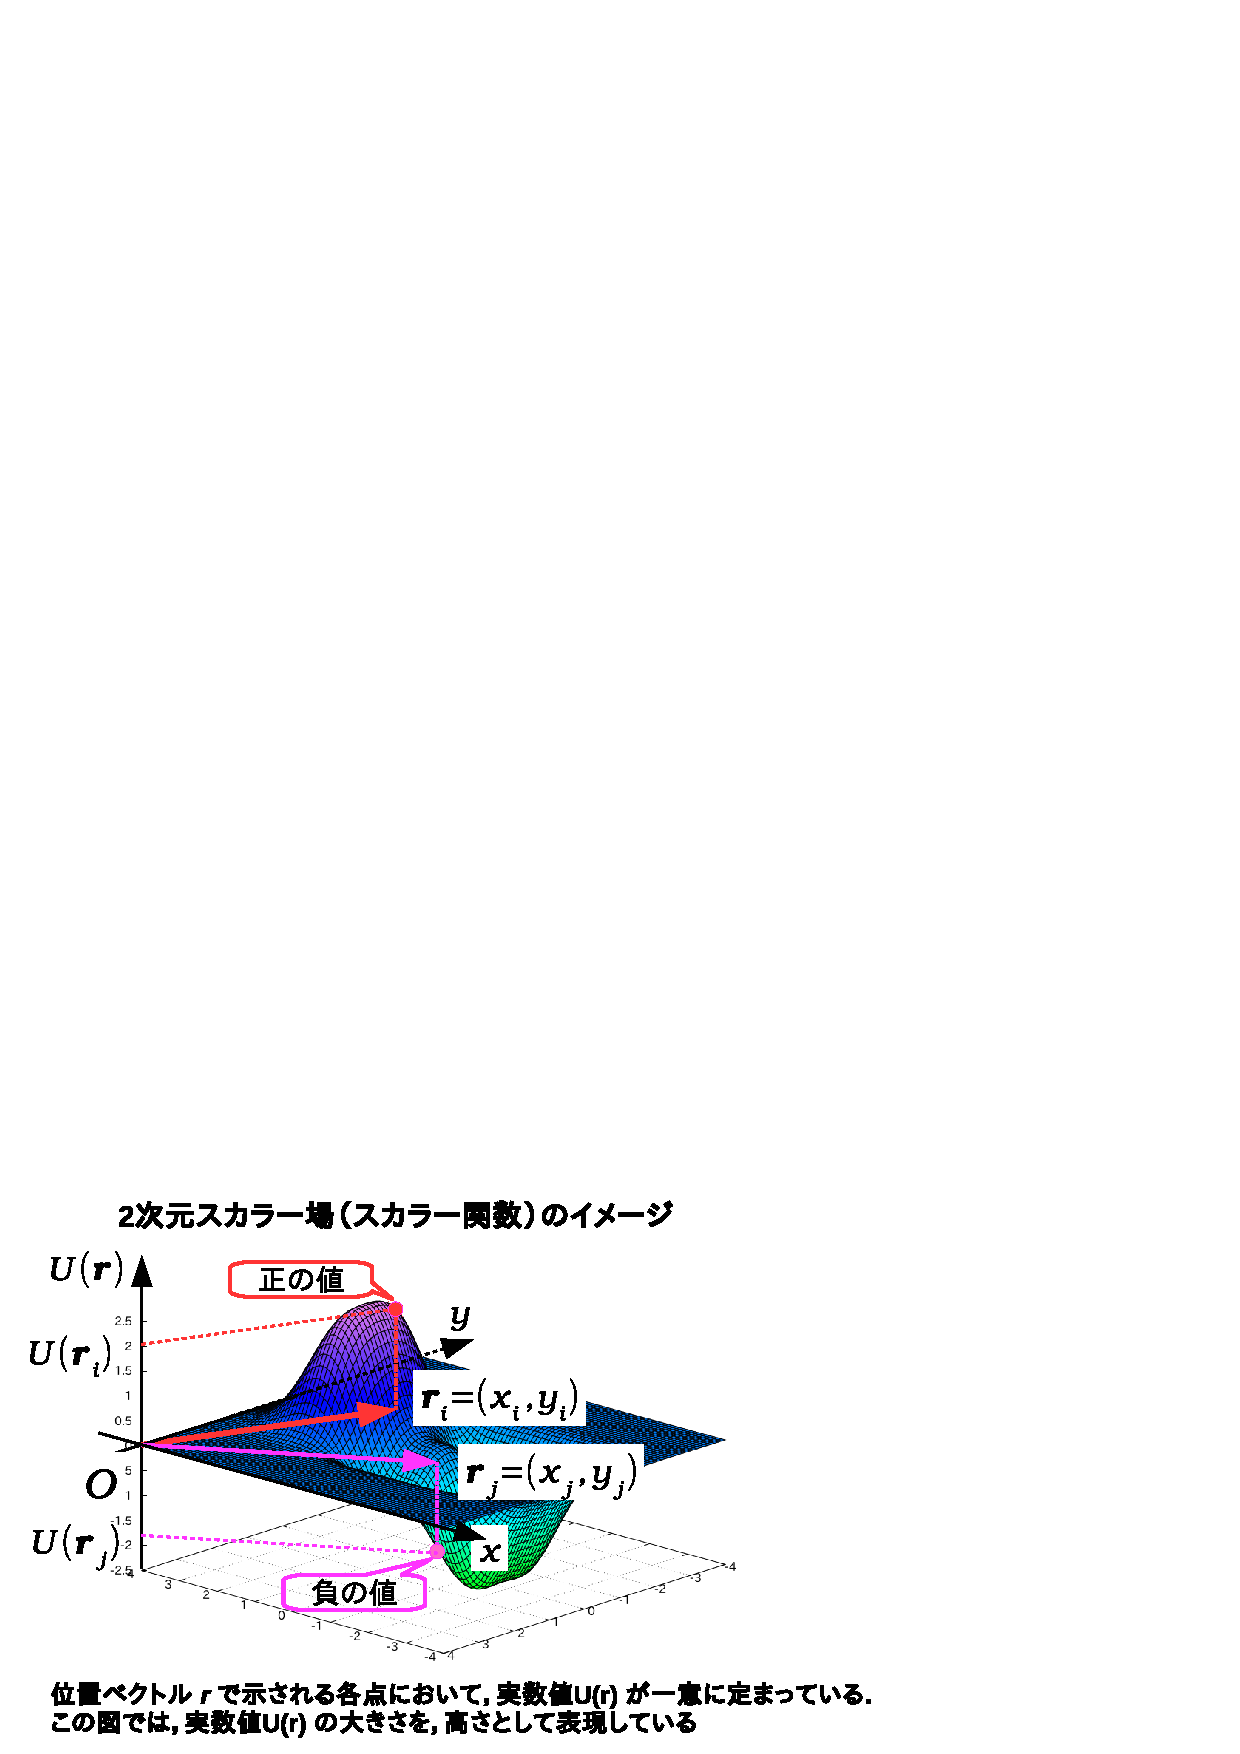
\includegraphics[keepaspectratio, width=7.2cm,height=6.64cm,clip]{scara_function_image001.pdf}
                            \caption{二次元のスカラー関数のイメージ}
                            \label{fig:scara_function_image001}
                        \end{center}
                    \end{figure}


                ポテンシャル$\cdot$エネルギーには地表付近の重力による
                位置エネルギー $mgh$ のほかに,もっと一般的な
                万有引力による位置エネルギーとか,
                電気的なポテンシャル$\cdot$エネルギーがある.
                ポテンシャル$\cdot$エネルギーといった時はこれらを総称していう時もあり,
                注意が必要である.
            \end{mysmallsec}

            \begin{mysmallsec}{運動エネルギーの定義}
                運動エネルギー $T$ についても,改めて定義する.
                    \begin{myshadebox}{運動エネルギーの定義}
                        運動エネルギー $T$ を,次式で定義する.
                        \begin{align}
                        T := \frac{1}{2}mv^{2}
                        \end{align}
                    \end{myshadebox}

                なぜ運動エネルギーというかについては,
                この式がエネルギーの単位をもち,かつ,速度だけによって
                その値が決まるからと考えればよいと思う.
            \end{mysmallsec}

            \begin{mysmallsec}{エネルギー関数 $E$ の独立変数}
                運動エネルギーは速度の関数として捉えられる
                    \footnote{
                        上で運動量表示もできることを示したが,ここでは速度表示の運動エネルギーを
                        考える.
                    }.
                これを,$T=T(\dot{\br})$ と表す.
                また同様に,ポテンシャル$\cdot$エネルギーは位置座標の関数として捉えることができ,
                これを $U=U(\br)$ と書く.
                従って,力学エネルギーは速度と位置の関数である考えられる.なぜなら,
                \begin{align}
                E(\dot{\br},\,\br)=T(\dot{\br})+U(\br)
                \end{align}
                と書けるからである.
            \end{mysmallsec}

            \begin{mysmallsec}{エネルギー保存則}
                さて,力学的エネルギー保存の法則を式(\ref{b})のように書いても
                よいが,「保存則」というからには,時間に依存していないということを
                式で表現しておきたい.そこで,上式の力学的エネルギー $E$ を時間微分して,
                その結果が 0 であるというように表現する形に書き換えておく.
                            \begin{myshadebox}{力学的エネルギー保存の法則}
                                力学的エネルギー保存の法則は,次式によって表される.
                                \begin{align}
                                    \frac{\df E}{\df t}=0
                                \end{align}
                            \end{myshadebox}

                このように考えられる理由は,物体の運動エネルギーとポテンシャル$\cdot$エネルギーの和 $E$ が
                時間変化しないという前提があるからである.
                物体の運動エネルギーと位置エネルギーが時間変化するとき,
                すなわち,$T=T(\dot{\br},\,t)$,$U=U(\br,\,t)$ であるとき
                は,一般には保存則は成り立たない.物体のエネルギーが時間変化するということは,物体は外か
                ら仕事を受けてエネルギーをもらう(とられる)からである.仕事とは外力が引き起こすものであり,
                つまり,「物体に外力が働くときには,力学的エネルギー保存の法則は成り立たない」とい
                える.式で書けば以下の通り.

                この場合の力学的エネルギーは時間 $t$ を変数に含み,
                \begin{align}
                E(\dot{\br},\,\br,\,t)
                =T(\dot{\br},\,t)+U(\br,\,t)
                \end{align}
                と書かれる.時間 $t$ で微分すると,
                \begin{align*}
                \frac{\rd E(\dot{\br},\,\br,\,t)}{\rd t}
                &=\frac{\rd }{\rd t}\biggl\{ T(\dot{\br},\,t)+ U(\br,\,t)\biggr\} \\
                &=\frac{\rd T(\dot{\br},\,t)}{\rd t}+\frac{\rd U(\br,\,t)}{\rd t}
                \end{align*}
                この式の最右辺は0ではなく,時間 $t$ を変数に含む関数である.これを
                簡単に $\alpha (\dot{\br},\,\br,\,t)$ と
                書くことにしよう.すると式は,
                \begin{align}
                \therefore \quad
                \frac{\rd E(\dot{\br},\,\br,\,t)}{\rd t}
                =\alpha (\dot{\br},\,\br,\,t)
                \end{align}
                というように,エネルギー保存則の時間微分は,時間に依存することがはっきりとわかる.

                この関数 $\alpha (\dot{\br},\,\br,\,t)$ の具体的な形は,
                運動エネルギーとポテンシャル$\cdot$エネルギーが
                どのように時間に依存しているかによる.
                この関数 $\alpha(\dot{\br},\,\br,\,t)$ が
                物体のエネルギーの変化量である.

                従って \textbf{外力が物体に働くとき,力学的エネルギーは
                保存しない} ということになる.しかし,もっと広く考えて,外力を含んだ系を
                考えるならば,エネルギーは保存している.これを \textbf{エネルギー保存の法則} という.
                この法則は経験的事実によって,与えられる法則であり,この法則が破られた現象は
                ないとされる.
                (この場合,力学的エネルギーが保存するわけではない.
                外力によって生じた熱力学的エネルギーや電磁気的エネルギーのことをいう.)
            \end{mysmallsec}

            \begin{mysmallsec}{まとめ}
                説明が長くなってしまったが,以上によって,ニュートンの運動方程式から,
                力学的エネルギー保存の法則を導いたことになる.整理しよう.
                まず,ニュートンの運動方程式を認めた($m\textit{\textbf{a}}=\bF$).これは
                力学の出発点となる方程式である.その次に,
                仕事という概念を導入し($W=\bF\cdot \Delta \textit{\textbf{s}}$),
                そこから力学的エネルギーという概念を,運動エネルギーと位置エネルギーの
                2種類のエネルギーの和であると定義した($E=T+U$).そして,
                力学的エネルギーは時間によらず一定値を保つことを
                発見した.

                従って,ニュートンの運動方程式から,
                力学的エネルギー保存の法則を見出したことになる.
            \end{mysmallsec}

            \begin{memo}{注意}
                但し,この $\bF$ は \textbf{保存力} であるとして
                いることを忘れてはならない.
                保存力については後の\ref{PF}で確認することだが,
                ここでは,「力のする仕事が経路によらず,始端と終点
                によってだけ決定されるならば,この力は保存力である」
                と考えてもらいたい.
            \end{memo}


%       %======================================================================
%       %  SubSection
%       %======================================================================
        \subsection{万有引力によるポテンシャル$\cdot$エネルギー}
            ポテンシャル$\cdot$エネルギーの定義を得たので,それを具体的に計算してみる.その例として,
            万有引力によるポテンシャル$\cdot$エネルギーを考える.
            ただ単に,ポテンシャル$\cdot$エネルギーの定義
            式(\ref{eq:PE})に,万有引力を代入すればよいだけである.では,
            早速計算する.

            万有引力は,式(\ref{Grav})によって
                \begin{align}
                    \bF_{\rm{AB}}
                    = -G\frac{m_{\rm{A}}m_{\rm{B}}}{{\left| \br_{A}
                    -\br_{B} \right|}^{2}}
                    \frac{\br_{A}-\br_{B}}{\left| \br_{A}
                    -\br_{B} \right|}
                \end{align}
            と書かれた.ここでは, 質量 $m_{\rm{A}}$ によるポテンシャル$\cdot$エネルギーを考える.
            式変形が煩雑にならないように,
                \begin{align*}
                \br:=\br_{A}-\br_{B}
                \end{align*}
            とおく.
                \begin{align}
                    \bF_{\rm{AB}}
                    = -G\frac{m_{\rm{A}}m_{\rm{B}}}{{\left| \br \right|}^{2}}
                    \frac{\br}{\left| \br \right|}
                \end{align}
            これを,ポテンシャル$\cdot$エネルギーの定義式(\ref{eq:PE})に代入すると,
                \begin{align}
                    U&=-\int \bF_{\rm{AB}}\cdot \df\br  \notag \\
                     &=\int G\frac{m_{\rm{A}}m_{\rm{B}}}{{\left| \br \right|}^{2}}
                    \frac{\br}{\left| \br \right|} \cdot \df\br \notag \\
                     &=Gm_{\rm{A}}m_{\rm{B}}\int \frac{1}{\left| \br \right|^{2}}\df\br \notag \\
                     \therefore \quad U
                     &=-Gm_{\rm{A}}m_{\rm{B}}\frac{1}{\left| \br \right|}
                \end{align}
            と計算される.
            $\br:=\br_{A}-\br_{B}$ を思い出せば,次のようになる.
                \begin{myshadebox}{重力ポテンシャル}
                    重力ポテンシャルは次式で定義される.
                    \begin{align}\label{eq:Grav_1}
                        U=-G\frac{m_{\rm{A}}m_{\rm{B}}}{\left| \br_{A}-\br_{B}\right|}
                    \end{align}
                \end{myshadebox}

            この式(\ref{eq:Grav_1})が質量 $m_{\mathrm{A}}$ が
            その周りに生じさせるポテンシャル$\cdot$エネルギーである.
            このようなポテンシャルを \textbf{重力ポテンシャル} いう.

%       %======================================================================
%       %  SubSection
%       %======================================================================
        \subsection{保存力}\label{PF}
                    今までは,力の存在を仮定して,エネルギーを考えていた.しかし,あくまで仮定しているだけであって,
                    決してはっきりとした概念ではない.ならば逆に,エネルギーを仮定して
                    力を導くことを考えてもよいだろう.
                    力とエネルギーのどちらを基礎とするかは,
                    理論がスマートになる方をとるべきだ.
                    エネルギーを仮定して,力を導出する方が現代的な考え方である.
                    ポテンシャル$\cdot$エネルギーの定義式を力 $\bF$ について
                    解く.$\bF=\left( F_{x}, F_{y},F_{z}\right)$ とする.
                    また,$\df\br=\left( \df x ,\df y ,\df z \right)$ とする.
                        \begin{align}
                            U &= -\int \bF\cdot \df\br \notag \\
                              &= -\int \left( F_{x}\df x+F_{y}\df y+F_{z}\df z \right)
                        \end{align}
                    ここで,$\rd U/\rd x$ を計算すると,
                        \begin{align}
                            \frac{\rd U}{\rd x}=-F_{x}
                        \end{align}
                    となる.ここで記号 $\rd U/\rd x$ の $\rd/\rd x$ は,
                    ($U$ を)“$x$ について微分する”ということである.その際,その他の変数($y$,$z$)は
                    定数とみなすと約束する.$x$ 方向の関数の変化度を知りたいときに,
                    用いる概念である.このような微分の仕方を \textbf{偏微分} という.

                    $y$,$z$ 方向についても同様に考えて,
                        \begin{align}
                        \frac{\rd U}{\rd y}&=-F_{y} \\
                        \notag \\
                        \frac{\rd U}{\rd z}&=-F_{z}
                        \end{align}
                    以上より,
                        \begin{align}\label{hozonryoku}
                            \left( \frac{\rd U}{\rd x} , \frac{\rd U}{\rd y},
                            \frac{\rd U}{\rd z}\right)
                            &=\left( -F_{x} , -F_{y} ,-F_{z} \right) \notag \\
                            \therefore \quad \bF
                            &=-\left( \frac{\rd U}{\rd x} ,
                            \frac{\rd U}{\rd y},
                            \frac{\rd U}{\rd z}\right)
                        \end{align}
                    を得る.ここで,次の微分演算子を定義する.
                        \begin{align}
                        \dgrad:= \left( \frac{\rd}{\rd x} , \frac{\rd}{\rd y},
                        \frac{\rd}{\rd z}\right)
                        \end{align}
                    (この記号の図形的なイメージは次項目で説明する.ここでは
                    とりあえず,記号として受けいれてほしい.)

                    この微分演算子は,$U$ の $x$,$y$,$z$ の3方向の傾きを求める演算子である.つまり,
                    空間の \textbf{勾配}
                        \footnote{
                            「勾配」とは,
                            面の傾斜の度合いのことをいう.例えば,道路の坂
                            が急であるとき,「この坂は急勾配である」といった使い方がされる.
                        }
                    を求める演算子と言える.$\dgrad$ を「グラディエント」と読む.
                    式(\ref{hozonryoku})を
                        \begin{align}
                            \bF=-\left( \frac{\rd}{\rd x} ,
                            \frac{\rd}{\rd y},
                            \frac{\rd}{\rd z}\right)U
                        \end{align} と変形する.そして,$\dgrad$ を
                    用いて,\\
                            \begin{align}
                                \bF=-\mathrm{grad\,} U
                            \end{align}
                    と書ける.
                    この式より,ポテンシャル$\cdot$エネルギーを仮定して力を導出するという意味として捉え直せる.

                    なので,ここで思い切って,保存力が生じている理由は,その周囲にポテンシャルエネルギーがあるからである,
                    と考えなおそう.保存力がポテンシャルエネルギーを周囲に作るというイメージよりも,そもそも最初は
                    ポテンシャルエネルギーがそこにあり,我々は,ポテンシャルエネルギーそのものを見ることはできないが,
                    その一端を保存力として観測していると考える方が,自然である.力を仮定してポテンシャルエネルギーを
                    導く場合には,試験用の質点を用意して至るところに置き,ポテンシャルエネルギーの分布を得るとになる
                        \footnote{
                                保存力を線積分するイメージ.
                        }.
                    しかし,ポテンシャルエネルギーを仮定すれば,ポテンシャルエネルギーの勾配($\dgrad$)を取るだけで,
                    保存力がえられるのだ.

                    こう考えなおすと,保存力 $\bF$ は,以下のように,ポテンシャルエネルギー $U(\br)$ の勾配で与えられる.
                        \begin{align*}
                                \bF = -\dgrad U(\br) = -\frac{\rd U(\br)}{\rd \br}.
                        \end{align*}
                                        両辺を始点 ${\br}_{\mbox{a}}$ から終点 ${\br}_{\mbox{b}}$ で積分すると,
                        \begin{align}\label{eq:forceF_and_potentialU}
                                   \int_{\br_{\mbox{a}}} ^{\br_{\mbox{b}}}\bF \cdot \br
                                   &=    \int_{\br_{\mbox{a}}} ^{\br_{\mbox{b}}}
                                           \left(
                                                -\frac{\rd U(\br)}{\rd \br}
                                           \right) \notag \\
                                   &=  - \int_{\br_{\mbox{a}}} ^{\br_{\mbox{b}}} \df U(\br) \notag \\
                                   &=  - \left( U(\br_{\mbox{b}}) - U(\br_{\mbox{a}}) \right) \notag \\
                                   &=  - U(\br_{\mbox{b}}) - ( - U(\br_{\mbox{a}}) ) \notag \\
                                   &=  \mbox{(一定)}
                        \end{align}
                    最初の位置 $\br_{\mbox{a}}$ でのポテンシャルエネルギー $-U(\br_{\mbox{a}})$ と移動後の位置 $\br_{\mbox{b}}$ の
                    ポテンシャルエネルギー $-U(\br_{\mbox{b}})$ の差のみで表せるという結果を得た.つまり,経路に依存していない.
                    どのような経路をとっても,始点と終点を指定するだけで,線積分が計算できるのだ,この線積分は位置と力の内積に
                    関するものであり,すなわち,始点から終点までになした仕事にほかならない,とどのつまり,の式は,
                    物体を $\br_{\mbox{a}}$ から $\br_{\mbox{b}}$ まで移動させるのに必要なエネルギーを表しているということだ.

                                        ただこのままでは,位置 $\br$ のポテンシャルエネルギーを $-U(\br)$ と書いた場合,終点は $-U(\br)$ だが始点が
                                        定まっていないため,値が定まらない.そこで,基準点を設けて,それに対するポテンシャルエネルギーを定義しよう.

                                        一般に,$A-B$ という式を見た場合,$A$ は $B$ を基準とした値であると解釈できる.例えば,$A=5$,$B=3$ とした時,
                                        $A-B=2$ であり,$A$ は絶対値5だけど $B$ から見ればその差は2である.
                                                \footnote{
                                                        このような見方を,$B$を基準にしてみると表現する
                                                }.
                                    同様に,$- U(\br_{\mbox{b}}) - ( - U(\br_{\mbox{a}}) )$ は $- U(\br_{\mbox{a}})$ を基準にしたときの,
                                    $- U(\br_{\mbox{b}})$ の値と解釈できる.そこで,$- U(\br_{\mbox{a}})=0$ となるような点
                                        \footnote{
                                                このような点が現実にあるわけでない.人間が勝手に基準となる点を設定しなければいけない.$- U(\br_{\mbox{a}})=0$ と
                                                できる点を適宜用意する必要がある.多くの場合は,無限遠点を基準点に取ることが多い.無限遠点とは,これまた曖昧な
                                                概念だが,ここから遠ざかって見えなくなった先の更に先というイメージで十分だ.
                                                実際,無限遠点はここだと示すことはできず,想像するより他にない.問題によっては基準点を別の点にとったほうが
                                                計算しやすい場合がある.その場合は,基準点を最も計算しやすい適切な点に再設定すれば良い.どうせ基準点は計算結果に
                                                影響しないのだから(基準点を決めないと不定積分になり不定性が残るが,基準点があれば定積分となり不定性はなくなる).
                                        }
                                    を基準点にとると,定義する.
                                    こうすることで,始点を暗黙裏に仮定することにより,毎回基準点を示すことなく,ポテンシャルエネルギーを考えることができる.
                                    ただ,基準点を示さないのが当たり前になってくると,ポテンシャルエネルギーがそもそも基準点をとるということを忘れがちであるので,
                                    この点は注意が必要だ
                                        \footnote{
                                                簡略化した記述は効率的だが,記述しないがゆえに見えなくなってしまうというジレンマがある.
                                                慣れれば(当たり前になれば)当然のこととして捉えられるが,なかなか難しい.
                                        }.
                                    このように,より簡略化した記述では,ポテンシャルエネルギーと保存力の関係式は以下のようになる
                                        \footnote{
                                                まず,式(\ref{eq:forceF_and_potentialU})で,始点は $-U(\br_{\mbox{a}})=0$ となる基準点を選ぶのであった.
                                                また,終点 $-U(\br_{\mbox{b}})$ の添字 $\mbox{b}$ も明示しなくても,常に終点を示すものであると読み取ることが可能なので,
                                                記述省略してしまおう.
                                        }.
                        \begin{align*}
                                   \int \bF \cdot \br  =  - U(\br)
                        \end{align*}

                    一般には,全ての力がポテンシャル$\cdot$エネルギーから導出されるわけではない.つまり,非保存力であるものもある.
                    この場合には,非保存力 $\bar{\bF}$ のする仕事を $W$ として,
                        \begin{align}
                            \bar{\bF}
                            = -\frac{\rd W}{\rd\br}
                        \end{align}
                    と書ける.もちろん,保存力と非保存力の両方を含む場合は,力の重ね合わせの原理から,
                        \begin{align}
                            \bF+\bar{\bF}
                            = -\frac{\rd U}{\rd\br}
                              -\frac{\rd W}{\rd\br}
                        \end{align}
                    である.
                    \begin{figure}[hbt]
                        \begin{center}
                            \includegraphicslarge{hozonryoku.pdf}
                            \caption{重力から受ける仕事は鉛直方向のみ}
                            \label{fig:hozonryoku}
                        \end{center}
                    \end{figure}

%       %======================================================================
%       %  SubSection
%       %======================================================================
        \subsection{勾配}
                    演算子 $\dgrad$ は,以下のように定義される量であることを,
                    前項目で確認した.
                        \begin{align}
                        \dgrad:= \left( \frac{\rd}{\rd x} , \frac{\rd}{\rd y},
                        \frac{\rd}{\rd z}\right)
                        \end{align}
                    この定義式をイメージすることが,この項目の目標である.

                    唐突ではあるが,
                    まず,連続でなめらかな1変数関数 $f_{1}=f(x)$ のグラフの接線の傾き $f'_{1}$ 考える.
                    $f'_{1}$ は $f_{1}$ の $x$ に関する微分であり,
                    \begin{align}
                    f'_{1}=\frac{\df }{\df x}f_{1}
                    \end{align}
                    のように与えられる.(図\ref{fig:grad1}参照)
                    これが1変数関数の場合である.

                \begin{figure}[hbt]
                    \begin{tabular}{cc}
                        \begin{minipage}{0.5\hsize}
                                    \begin{center}
                                        \includegraphicsdouble{grad1.pdf}

                                        (A) 1変数関数
                                        \label{fig:grad1}
                                    \end{center}
                        \end{minipage}
                        \begin{minipage}{0.5\hsize}
                                    \begin{center}
                                        \includegraphicsdouble{grad2.pdf}

                                        (B) 2変数関数
                                        \label{fig:grad2}
                                    \end{center}
                        \end{minipage}
                    \end{tabular}

                        \caption{傾き}
                \end{figure}

                    この考えを,
                    2変数関数 $f_{2}=f_{2}(x,\,y)$ の場合について拡張してみる.
                    関数 $f_{2}=f_{2}(x,\,y)$ は図\ref{fig:grad2}のように
                    描くことができる.もちろん,関数 $f_{2}=f_{2}(x,\,y)$ は連続で
                    なめらかであることを仮定している.関数 $f_{2}=f_{2}(x,\,y)$ を,
                    点$(x,\,y)$ を代入したときの高さを表していると考えれば,
                    このような点を全て集めると,
                    それは\textbf{曲面}をなしていると言える
                        \footnote{
                            つまり,$f(x,\,y)$ は幾何学的には,曲面を表す関数としてイメージされる.
                        }.
                    1変数関数における曲線が,
                    2変数関数になると,曲面になるのである.
                    従って,2変数の場合には,
                    直線の接線の傾きを考えるのでは不十分であり,
                    面の \textbf{勾配} を考えなければいけない
                        \footnote{
                                「勾配」とは面の傾き具合を表す語彙.1次元の場合は「傾き」という
                                表現を使ったが,2次元の場合は「勾配」と言い表す.2次元以上の場合
                                でも「勾配」という.
                        }.
                    そこで,図\ref{fig:grad2}の青い線で描いたような,
                    接面の勾配を考えるのである.この接面の勾配を考える.
                    図\ref{fig:grad2}では説明しにくいので,改めて,
                    図\ref{fig:grad3}に必要な部分だけ書き改めることにする.
                    (若干異なっているが許してほしい.)

                \begin{figure}[hbt]
                    \begin{tabular}{cc}
                        \begin{minipage}{0.5\hsize}
                                    \begin{center}
                                        \includegraphicsdouble{grad3.pdf}

                                        (A) 2変数関数の傾き
                                        \label{fig:grad3}
                                    \end{center}
                        \end{minipage}
                        \begin{minipage}{0.5\hsize}
                                    \begin{center}
                                        \includegraphicsdouble{grad4.pdf}

                                        (B) 接面の勾配
                                        \label{fig:grad4}
                                    \end{center}
                        \end{minipage}
                    \end{tabular}

                        \caption{面の傾き}
                \end{figure}

                図の緑の太線で示した曲面部分に接する平面を
                考える.図の $A$ は $x$--$y$ 平面上の点を表している.そのような平面のことを \textbf{接面} と
                いうことにする.この接面の勾配を
                示すには,$x$ 方向の接面の傾きと,$y$ 方向の
                接面の傾きを考えればよい.従って,それぞれの方向に \textbf{偏微分} すればよい.
                前項目では偏微分の定義には触れなかったので,
                ここでは簡単に偏微分の定義式を示しておこうと思う.

%       %======================================================================
%       %  SubSection
%       %======================================================================
        \subsection{保存力と $\dgrad$ の図的イメージ}
                偏微分は,グニャグニャ曲がっている面のある一点における
                傾きを計算する場合に役に立つ.面の傾きを考えるには,
                2つの方向の傾きを考える必要がある.しかし,2方向の傾き
                を同時に考えることは難しい.そのため,一方向ずつ傾きを
                計算する.一方向の傾きを計算するには,曲線の傾きと
                同じように考えられる.そのとき,残りのもう1方向は定数として
                扱う.

                例えば,接面の $x$ 方向の傾きを考える場合,$y$ 座標を一時的に固定して定数と
                して扱い,$x$ 方向のみに着目し微分する.偏微分の記号は通常の微分と区別するために,
                $\rd$ という文字が使われる.具体的には,以下の通り.
                \begin{align}
                    \frac{\rd }{\rd x}f(x,\,y) := \lim_{\Delta x \to 0} \frac{f(x+\Delta x,\, y) - f(x,\,y)}{\Delta x}.
                \end{align}

                接面の $x$ 方向の傾きも同様に考えて,
                \begin{align}
                    \frac{\rd }{\rd y}f(x,\,y) := \lim_{\Delta y \to 0} \frac{f(x,\,y+\Delta y) - f(x,\,y)}{\Delta y}.
                \end{align}

                これらを用いて,曲面f上の点($x,\,y$)の接面は
                    \begin{equation*}
                        \left( \frac{\rd }{\rd x}f(x,\,y) \,,\; \frac{\rd }{\rd y}f(x,\,y) \right)
                    \end{equation*}
                と表現できる.ただ,$f$ の独立変数をいちいち書いていると煩雑なので,省略する場合が多い
                    \footnote{
                        偏微分の対象となる方向は分母でわかるし,他の変数は定数扱いなので無理して明示する必要もない.
                        問題になるとしたら,独立変数の個数がわからなくなってしまうことだが,前もって明記しておけば
                        覚えていられるだろう.
                    }.
                    \begin{equation*}
                        \left( \frac{\rd }{\rd x}f \,,\; \frac{\rd }{\rd y}f \right)
                    \end{equation*}
                もっと省略して,以下のように書かれることもある($f$ をカッコの外に出した).
                    \begin{equation*}
                        \left( \frac{\rd }{\rd x} \,,\;  \frac{\rd }{\rd y} \right) f
                    \end{equation*}
                こうすると,式に意味を与えやすい
                    \footnote{
                        ただし,注意したいのは,
                        $\displaystyle \left( \frac{\rd }{\rd x} \,,\; \frac{\rd }{\rd y} \right)$ と $f$ の積
                        と解釈してはいけない,ということである.
                    }.
                こうすると,表現上,$f$ に対して
                操作 $\displaystyle \left( \frac{\rd }{\rd x} \,,\; \frac{\rd }{\rd y} \right)$ を施すことで,
                接面が現れると読むことができる.物理学では,
                    \begin{equation*}
                        \dgrad := \left( \frac{\rd }{\rd x} \,,\; \frac{\rd }{\rd y} \right)
                    \end{equation*}
                として,単に
                    \begin{equation*}
                        \dgrad f
                    \end{equation*}
                と書かれる.ポテンシャルエネルギーを考える場合には,$f=-U(\br)$ とすればいい.

                    ポテンシャルエネルギーの関数 $U(\br)$ が与えられている時,保存力 $\bF(\br)$ は以下のように計算できる.
                    \begin{align*}
                        \bF (\br) &= - \dgrad U(\br) \\
                                  &= -\left(
                                                \frac{\rd}{\rd x}\,,\;
                                                \frac{\rd}{\rd y}\,,\;
                                                \frac{\rd}{\rd z}
                                     \right)  U(\br) \\
                                  &=  \left(
                                        - \frac{\rd U(\br)}{\rd x}\,,\;
                                        - \frac{\rd U(\br)}{\rd y}\,,\;
                                        - \frac{\rd U(\br)}{\rd z}
                                     \right)
                        \end{align*}

                上式で表されるポテンシャルエネルギーと保存力のイメージを,以下に表現しておこう.
                    \begin{figure}[hbt]
                        \begin{center}
                            \includegraphicslarge{scara_function_image002.pdf}
                            \caption{ポテンシャルエネルギーと保存力}
                            \label{fig:sensekibun_shukaisekibun_002}
                        \end{center}
                    \end{figure}

                この図で注意してみて欲しいのは,ポテンシャルエネルギーを2次元で表していることである.
                実際の空間はは3次元だが,これだと図に表すことができない
                        \footnote{
                            関数の取る値をグラフで示すための次元が1つ必要になるからである.
                            ここでは,本来の3次元の内から1次元減らし,代わりに関数のとる
                            値を山として表現している.
                        }.

%       %======================================================================
%       %  Memo
%       %======================================================================
        \begin{memo}{$\rd / \rd \br$ という表現について}
            上で使ってしまったが,便利でよく使われてしまう表現に,
                        \begin{equation*}
                                \frac{\rd f(\br)}{\rd \br}
                        \end{equation*}
            というものがある.

            ベクトル $\br$ で割り算しているように見えるが,そうではない
                \footnote{
                    "ベクトル除算" なんてものはない.
                }.
            本当は,
                        \begin{align*}
                                \frac{\rd f(\br)}{\rd \br}
                                &=
                                    \left(
                                      \frac{\rd f(\br)}{\rd x} \,,\;
                                      \frac{\rd f(\br)}{\rd y} \,,\;
                                      \frac{\rd f(\br)}{\rd z}
                                \right) \\
                                &=
                                    \left(
                                      \frac{\rd f(x,\,y,\,z)}{\rd x} \,,\;
                                      \frac{\rd f(x,\,y,\,z)}{\rd y} \,,\;
                                      \frac{\rd f(x,\,y,\,z)}{\rd z}
                                \right)
                                \end{align*}
                    という意味で使われるものである.紛らわしいが,よく見かける表現なので注意しておきたい.
                    こういう表現は,疑問や誤解を招くので,避けたほうが良い
                        \footnote{
                            勾配演算子 $\dgrad$ や後で紹介する数学記号 $\nabla$ を使って表現すべき.
                        }.
        \end{memo}

%       %======================================================================
%       %  SubSection
%       %======================================================================
        \subsection{保存力と周回積分}\label{subsec:hozonryoku_to_shukaisekibun}
                        ポテンシャルエネルギー $U(\br)$ のみの場合などのように,外力が働かない時,
                        始点Aと終点Bの2つの位置ベクトルを定めると,AからBまでの経路Cは無数に存在するが,
                        AからBまで物体を移動させる仕事はその経路に依存せず,一定値をとる.
                        \begin{equation*}
                                \oint_{\mbox{C}} \bF (\br) \cdot \df \br = U(\br_{\mbox{b}}) - U(\br_{\mbox{a}}).
                        \end{equation*}
                        このような性質を持つ関数で表される力のことを,\textbf{保存力} と言うことはすでに記述した.
            特に注目すべきはことは,B$=$Aとした時(始点と終点を同じ点にした場合),
                        \begin{equation*}
                                \oint_{\mbox{C}} \bF (\br) \cdot \df \br = U(\br_{\mbox{a}}) - U(\br_{\mbox{a}}) = 0
                        \end{equation*}
                        となることである.


                        ポテンシャルエネルギー値 $U(\br)$ がベクトル $\br$ に対して一意に定まる場合,
                        $U$ により生じる力は保存力となる.
                    \begin{figure}[hbt]
                        \begin{center}
                            \includegraphicslarge{sensekibun_shukaisekibun_001.pdf}
                            \caption{保存力の性質}
                            \label{fig:sensekibun_shukaisekibun_001}
                        \end{center}
                    \end{figure}


                        しかし,例えば下図のように,ポテンシャルエネルギー値 $U(\br)$ がベクトル $\br$ に対して
                        一意に\textbf{定まらない}場合,$U$ により生じる力は保存力ではない.
                    \begin{figure}[hbt]
                        \begin{center}
                            \includegraphicslarge{sensekibun_shukaisekibun_004.pdf}
                            \caption{保存力でない場合}
                            \label{fig:sensekibun_shukaisekibun_004}
                        \end{center}
                    \end{figure}

%   %==========================================================================
%   %  Section
%   %==========================================================================
    \section{エネルギーと運動量}
        エネルギーと運動量は似たような概念だ.この2つの間には大切な関係がある.
        特に,量子力学を学習するとこの関係が顕著に現れてくる.
        運動量 $\bp$ をもつ物体に関与する力を保存力とし,$\bF$ とする.
                \footnote{
                        ここでは保存則について考えているのであった.保存力以外の外力が
                        働く場合は,運動量保存則とエネルギー保存則は成立しないの.
                }.
        運動量表示の運動方程式は
                        \begin{align*}
                        \frac{\df \bp}{\df t} = \bF.
                        \end{align*}
        であった.$t$ は時間である.
        ところで,保存力である $\bF$ はポテンシャルエネルギー $U(\br)$ を導入すると,
                        \begin{align*}
                        \bF = -\frac{\rd U}{\rd \br}.
                        \end{align*}
        ここで,$E(\br)=-U(\br)$ と置いてしまおう.
                        \begin{align*}
                        \bF = \frac{\rd E}{\rd \br}.
                        \end{align*}
                要するに,$\rd U/\rd \br$ と $\rd E/\rd \br$ は共に力の次元を持っている,
                $\bF$ を消去して,それぞれの次元を考えると,
                        \begin{align*}
                        \left[\frac{\df \bp}{\df t}\right] = \left[\frac{\rd E}{\rd \br}\right]
                        \end{align*}
                微分記号と偏微分記号は不要.
                        \begin{align*}
                        \frac{[\bp]}{[t]} = \frac{[E]}{[\br]}
                        \end{align*}
                これを以下のように書きなおす.
                        \begin{align}
                                [\bp] \cdot [\br] = [E][t].
                        \end{align}
            もしかしたら,$\br=(x,\,0,\,0)$,$\bp=({p}_{x},\,0,\,0)$ としたほうがわかりやすいかもしれない.
                        \begin{align*}
                                {p}_{x}x = Et.
                        \end{align*}

